\documentclass[a4paper, 12pt, oneside]{book}
\usepackage[top=1in,bottom=1in,left=1.25in,right=1.25in]{geometry}


\usepackage{fontspec,xltxtra,xunicode}
\usepackage[slantfont,boldfont]{xeCJK}

\usepackage[sort&compress,longnamesfirst]{natbib}

\usepackage{pdfpages}
%\usepackage{fancyhdr}
\usepackage{layout}
\usepackage{xCJKnumb}
\usepackage{titlesec} % 改变章节标题格式
\usepackage{indentfirst} % 首段缩进
\usepackage{thesis_cx}
\usepackage{natbib}
\usepackage{url}
\usepackage{graphicx}
\usepackage{epstopdf}
\usepackage{algorithm} % 算法排版
\usepackage{algpseudocode}
\usepackage{multirow}
\usepackage{titletoc}
\usepackage{float}
\usepackage{tabularx}

% \usepackage{subfigure}
\usepackage{subfig}
\usepackage{tikz}
\usetikzlibrary{fit,positioning}
\usepackage{amsmath}
\usepackage{amssymb}


%-----------------设置字体-------------------
%\setCJKmainfont{SimSun}
%\setCJKmainfont[BoldFont={STHeiti},ItalicFont=STKaiti]{STSong}

\newcommand{\tn}{\tabularnewline} %表格



\begin{document}
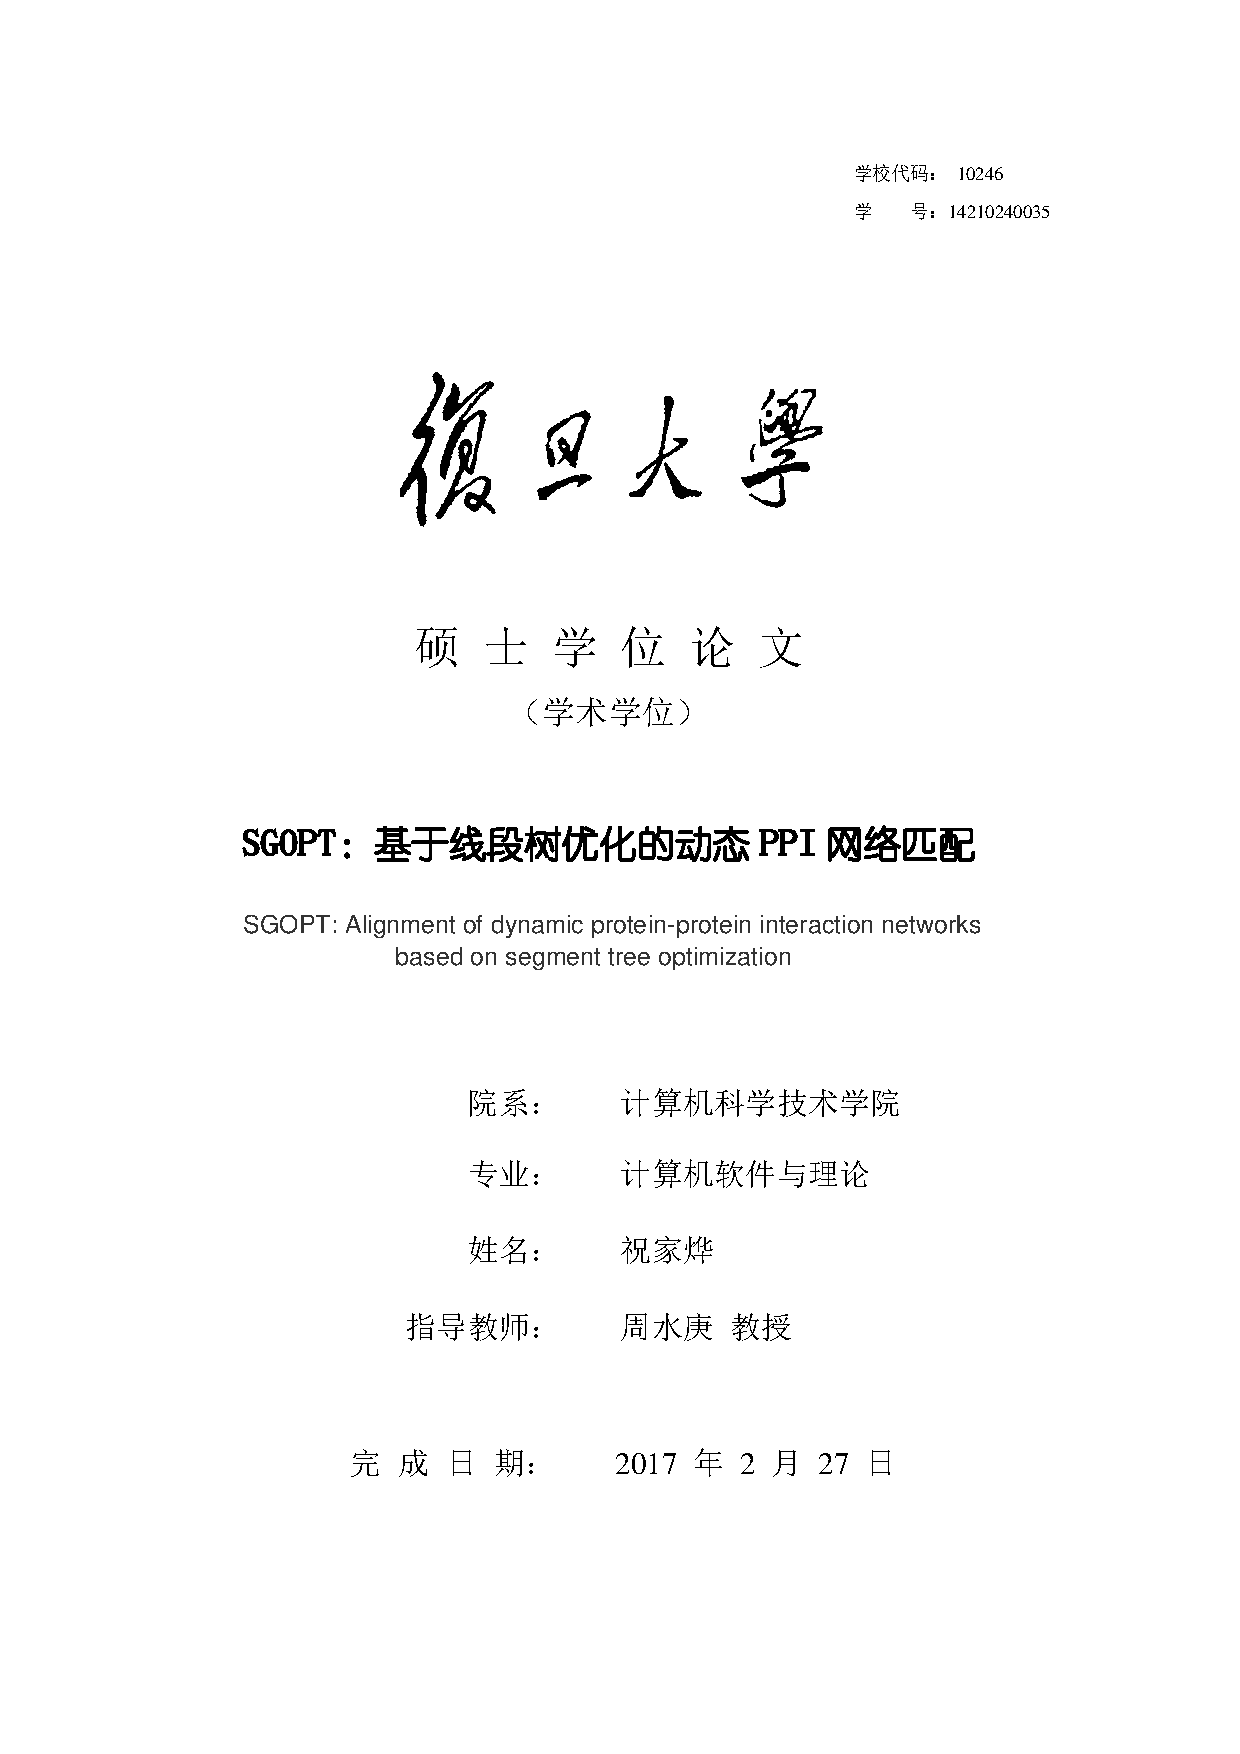
\includepdf{cover.pdf}

\pagenumbering{roman}

\newpage
\begin{titlepage}
\vspace*{120pt}
\centerline{\Huge 指导小组成员名单}
\vspace*{60pt}
\centerline{\Large 周水庚 \hspace*{10pt} 教授}
\end{titlepage}

%\song
\lhead{复旦大学硕士学位论文}
\rhead{目录}

%\song
\tableofcontents
\newpage

\pagenumbering{arabic}
%\song

\chapter*{摘要}
\addcontentsline{toc}{chapter}{摘要}
\rhead{摘要}
生物蛋白质相互作用网络,简称PPI网络(protein-protein interaction networks),是一种生物信息学中用来表示蛋白质之间相互作用关系的图模型,通过对PPI网络进行分析,可以得到许多和该生物的蛋白质相关的信息。而通过对不同物种间PPI网络进行网络匹配(alignment of PPI networks)的方法,则可以将一种生物PPI网络中已建立起的知识体系,转移到另一种未建立完整知识体系的生物PPI网络中。而其中,PPI网络匹配算法的好坏则起到了举足轻重的作用。

另一方面,由于大量基因表达数据(gene expression data)的存在,动态PPI网络的概念(dynamic protein-protein networks)被提出,这对既有的静态PPI网络匹配算法来说无疑是一种新的挑战。对于现有的匹配算法,环境从原来的静态PPI网络,变成了动态PPI网络,那么无论是匹配的概念,亦或是匹配好坏的衡量标准(measure alignment quality),都需要在动态PPI网络这一新环境下重新定义。

本文提出了动态PPI网络匹配的概念(alignment of dynamic PPI networks),定义了动态PPI网络匹配的问题和衡量标准,并且设计了一种在该问题下,能够提高既有静态PPI网络匹配算法在动态PPI网络中匹配效果的算法SGOPT(SeGment tree OPTimization)。SGOPT算法可以在既有静态匹配算法的基础上,通过一种局部调整的策略,利用线段树(segment tree)来高效地维护动态PPI网络中的匹配结果。SGOPT算法最终能够产生比既有静态PPI网络匹配算法更好的匹配效果,本文通过实验证明了其优势。


\noindent{\bf 关键词}:蛋白质相互作用网络,PPI,PPI网络匹配,PPI网络匹配算法,动态PPI网络,线段树,SGOPT


\chapter*{Abstract}
\addcontentsline{toc}{chapter}{Abstract}
\rhead{Abstract}

Protein-protein interaction networks are very important graph models which can reveal the relationship between proteins in a species. One can get much knowledge about proteins of the species by analyzing the PPI networks. Through the alignment of PPI networks, biological knowledge can be transferred between different species. Therefore, the goodness of the network alignment algorithms is very important.

On the other side, with much gene expression data, the concept of dynamic PPI networks is proposed which is obviously a new challenge to state-of-the-art static network alignment algorithms. The new concepts of alignment and alignment quality measurement, need to be defined when the condition changes from static PPI networks to dynamic ones.

This paper proposes the concept of alignment of dynamic PPI networks, defines the measurements of alignment quality, and designed an algorithm called SGOPT(SeGment OPTimization) which can be used to improve any alignment results produced by state-of-the-art static alignment algorithms. SGOPT maintains alignment by adjusting alignment locally and through a data structure called segment tree in environment of dynamic PPI networks. SGOPT finally can produce better alignments then state-of-the-art ones which is proved through systematic experiments in this paper.
\bigskip
\bigskip

\noindent{\bf Keywords}: protein-protein interaction networks, algorithms of alignment of PPI networks, dynamic PPI networks, segment tree, SGOPT
\newpage

\rhead{引言}
\chapter{引言}
%@@@@@@@@@@@@@@@@@@@@@@@@@@@@@@@@@@@@@@@@@@@@@@
\section{研究背景及意义}
生物学研究的一个重要目标,就是理解生命细胞中各个组成部分的功能以及它们之间的联系。其中,蛋白质(protein)是具有极其重要意义的生物结构,它能帮助我们理解细胞作用的机理。分析蛋白质序列以及比较不同蛋白质之间的序列相似性,都能帮助我们充分理解蛋白质的功能及作用。

但是,近年来,蛋白质被发现其往往不是单一活动的。生物的细胞生命活动,是需要许多蛋白质在一起相互作用,才能够完成的,而并不是靠某个单一的蛋白质就能做到的。发现并理解蛋白质与蛋白质之间的相互作用(protein-protein interactions,PPIs),就成为了领域内的重要课题之一。

伴随着这一新课题,许多新的生物学实验\cite{uetz2000comprehensive,ito2001comprehensive,krogan2006global,han2004evidence,nabieva2005whole,yook2004functional}被设计了出来,这些实验的目的便是发现蛋白质之间的相互作用结构。而这些大量的实验结果,急需一个合适的数学模型来对它们进行建模,以便于学者们的与实验与分析。

因此,学者们就提出了蛋白质相互作用网络(protein-protein interaction networks)这一图论模型。在有了PPI网络这一模型后,类似于通过匹配不同基因组序列以分析基因组的方法,通过匹配两种生物间的PPI网络,也能够成为分析生物细胞体内蛋白质相互作用的一种方法。而且,PPI网络之间的匹配,不但能够利用生物蛋白质之间的序列相似性,也能够利用网络之间的拓扑结构相似性,比起之前单一比较蛋白质序列相似性的方法,要好的多。

PPI网络匹配(PPI network alignment,NA)是将两个不同物种的PPI网络进行匹配的过程。NA的目的在于找到两个PPI网络中极为相似的一些区域,这个相似,从不同的研究问题来看,可以有不同的意义,可以是生物功能的相似,也可以是拓扑结构的相似。但无论是哪种相似的定义,PPI网络匹配的好坏,具有极其重要的的作用。一个好的PPI网络匹配,能够找到两个PPI网络中十分相似的子结构,从而能够把一种生物的知识体系,完全借鉴在另一种未知PPI网络中。而一个不好的PPI网络匹配,则没有这样的效果。

然而坏消息是,从图论学来看,PPI网络匹配涉及到的一个子问题,便是图论中经典的子图同构问题(subgraph isomorphism problem)。这一问题已经被证明是NP-完全问题,即没有已知的任何一种高效的算法能够完全解决这个问题。所以对于PPI网络的匹配,不能在有限时间内求出最优的解。

然而不同于子图同构问题的是,PPI网络匹配的目标,并不是完全的子图同构,而是找到尽可能相似的子图,这就给许多启发式的算法(heuristic algorithms)提供了契机。

而现在,大量的PPI网络数据与日俱增\cite{breitkreutz2008biogrid,hulovatyy2014revealing},这就要求更快,更好的PPI网络匹配算法。一个好的PPI网络匹配算法具有极其重要的意义。

%@@@@@@@@@@@@@@@@@@@@@@@@@@@@@@@@@@@@@@@@@@@@@@@@@
\section{研究内容}
一个PPI网络可以看成是图论中的一个图(graph),其中,每个蛋白质由一个点(node)表示,而蛋白质与蛋白质之间的相互作用关系,则可以看成这个图中的边(edge),至于这个边是否带权重,则取决于研究额问题。因此,PPI网络匹配其实就是对两个图作匹配的过程,而目的则是尽可能找出两个图中相似的子结构。由于寻找一个图在另一个图中的同构子图是一个NP-完全的问题\cite{cook1971complexity},因此,想要找到一个PPI网络在另外一个PPI网络中的完全等价子图是不可能的,我们只能期望找到尽量相似的子图。

从一般意义上来讲,网络匹配就是将两个网络的点进行匹配,使得所匹配的两个子图,具有极高的相似程度,而这个相似度,不但可以从网络的拓扑结构上来考虑,也可以同时考虑蛋白质之间的序列相似性。

网络匹配,主要分为局部网络匹配(local network alignment,LNA),和全局网络匹配(global network alignment)。一开始,LNA是人们关注的重点,它的目的在于找到两个网络中局部高度匹配的区域(highly conserved region),其产生的结果往往是两个网络中规模较小的子图,同时,一个源网络(source network)中的点可能会匹配多个目标网络(target network)中的点。

\begin{figure}[htbp]
\centering
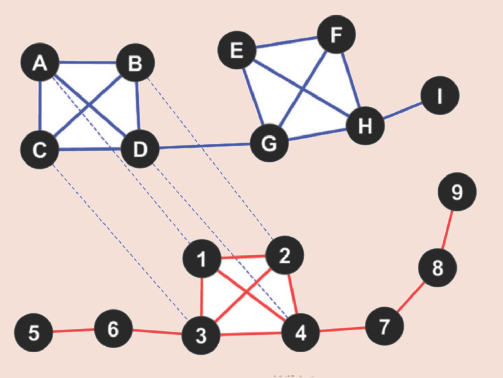
\includegraphics[height=0.25\textheight]{pic/lna.png}
\captionsetup{margin=50pt}
\caption{局部网络匹配,其中[1,2,3,4]可以和[A,B,C,D]匹配,也可以和[E,F,G,H]匹配 \cite{atias2012comparative} \label{fig:lna}}
\end{figure}
而全局匹配,顾名思义,则是从整体上来对一个网络进行匹配,它匹配的不是一个网络的子图,而是整个网络,并且,点与点之间的关系是一对一(one-to-one),而不是像LNA是多对多(many-to-many)。

\begin{figure}[htbp]
\centering
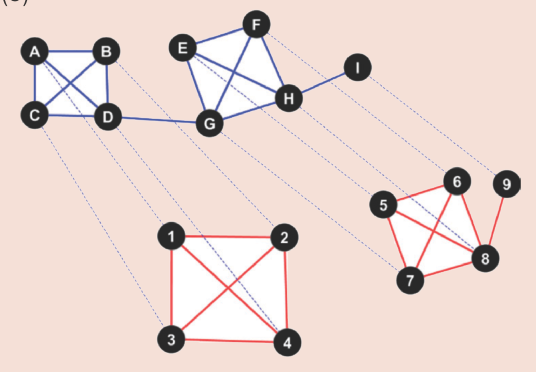
\includegraphics[height=0.25\textheight]{pic/gna.png}
\captionsetup{margin=50pt}
\caption{全局网络匹配,可以看到所有点都得到了匹配 \cite{atias2012comparative} \label{fig:gna}}
\end{figure}
相比于LNA注重两个网络中的局部相似性,GNA更关心一个网络在整体上和另一个网络的相似程度,近来越来越得到学者们的关注。

常见的局部网络匹配算法有PathBLAST\cite{kelley2004pathblast},NetworkBLAST\cite{sharan2005conserved},NetAlign\cite{liang2006netalign},MaWISh\cite{koyuturk2006pairwise}和Graemlin\cite{flannick2006graemlin}。之后,大量的全局网络匹配算法被提出,常见的有IsoRank\cite{singh2008global,liao2009isorankn},GRAAL\cite{kuchaiev2011integrative,malod2015graal,kuchaiev2010topological,milenkovic2010optimal,memivsevic2012c},MAGNA和MAGNA++\cite{saraph2014magna,vijayan2015magna++},SPINAL\cite{aladaug2013spinal},PINALOG\cite{phan2012pinalog},Netcoffee\cite{hu2013netcoffee},BEAMS\cite{alkan2014beams}。而本文研究的重点也是全局网络匹配。

IsoRank\cite{singh2008global}可以说是全局匹配算法中的先驱,它定义了两个网络间任意点对之间的相似度分数(score),这个分数由这个两个点代表的蛋白质的结构信息(structural similarity)和序列信息(protein sequence similarity)同时决定。然后以这个分数为标准,通过一定的策略,得到最终的匹配结果。类似于IsoRank,GRAAL一系列方法也定义了两个点之间的相似程度,不过不同于IsoRank的是,GRAAL一系列算法通过衡量两个点之间的小图度数相似度(graphlet-degree)作为两个点之间的相似度分数。GRAAL\cite{kuchaiev2010topological}是这一系列方法中的第一个方法,它根据计算得到的相似度分数,从高到低选择种子点对(seed pair),然后考虑这个点对的邻居集合(neighbour set)间的相似度,贪心地选择新的匹配点对。H-GRAAL\cite{milenkovic2010optimal}则用了二分图和匈牙利算法来优化GRAAL中的贪心过程,使得产生的匹配结果更好,而代价就是运行时间的增加。而MI-GRAAL\cite{kuchaiev2011integrative}则可以用不同的相似度分数来进行点对匹配。L-GRAAL\cite{malod2015graal}则是GRAAL系列算法中最近提出来的算法,它将图匹配的问题建模成了一个线性规划的问题,然后从该问题中得到一个较优的解。SPINAL算法\cite{aladaug2013spinal}是一种迭代式算法,它通过不断扩展已匹配点周围的邻居点对来生成新的匹配点对。MAGNA\cite{saraph2014magna}则运用了遗传算法来对已有匹配结果进行改进。

到目前为止,既有的网络匹配算法,无论是局部网络匹配算法还是全局网络匹配算法,都是针对静态PPI网络的匹配。也就是说,待匹配的目标网络是单一不变的。然而,生物细胞中的生命活动往往是动态的,而与细胞生命活动息息相关的蛋白质相互作用网络,其实是随时间变化的,可能在前一时刻两者还有相互作用的蛋白质,在后一时刻由于细胞生命活动的变更,而变得没有相互作用了。虽然将生物体蛋白质之间的相互作用以一个静态的PPI网络进行建模,已经能够体现蛋白质之间的相互作用了,但是这种表示方式并不能体现时间维度上的特征。

最近,关于动态PPI网络上(dynamic protein-protein interaction networks)的课题越来越多,预示着学者们对动态PPI网络的重视逐日增加。因此,为了更好地挖倔PPI网络的动态信息,在动态PPI网络上作PPI网络匹配是很有意义的一个新课题。虽然有不少文章的工作是基于动态PPI网络的\cite{lin2010dynamic,chen2014identifying,wang2013construction},但它们构造动态PPI网络的方式也不尽相同,而且研究的问题也不同。故针对本文研究的问题,我们需要一个完整的动态PPI网络概念以及对应的匹配问题的定义。

随之而来的问题就是,针对动态的PPI网络,能否提出切实有效的匹配算法呢?这也是本文要研究的重点内容。

本文首先提出了动态PPI网络的概念,然后定义了动态PPI网络匹配(alignment of dynamic protein-protein interaction networks)这一全新的问题,最后设计了一种算法叫SGOPT(SeGment tree OPTimization),并用完整的,系统的实验证明了该算法的效果。SGOPT是一种基于既有静态PPI网络匹配算法的方法,它是一种迭代式地,不断更新当前解的,基于局部调整策略的算法。它可以和任意既有静态PPI网络匹配算法相结合,产生更优秀的匹配。
%@@@@@@@@@@@@@@@@@@@@@@@@@@@@@@@@@@@@@@@@@@@@@@@@@@@@@@@@@@@
\section{本文结构}

第二章着重介绍了一些本文要研究的问题的相关概念,以及一些相关工作。第三章介绍了本文的主要贡献,包括动态PPI网络概念的定义,问题的定义,SGOPT算法的详细介绍等。第四章是实验分析部分。第五章总结文章。

\rhead{相关概念与相关工作介绍}
\chapter{相关概念与相关工作介绍}

%@@@@@@@@@@@@@@@@@@@@@@@@@@@@@@@@@@
\section{相关概念介绍}
本节主要对本文中经常出现的一些概念作相关介绍以及形式化的定义。

\subsection{PPI网络}
蛋白质相互作用网络(protein-protein interaction networks),简称PPI网络,是一种生物体内表示蛋白质相互之间作用的模型。定义图$G=(V,E)$为一个PPI网络,其中$V$是点集,其中每个点代表一种蛋白质,$E$是一个$V×V$的边集,一条边$(u,v)$代表蛋白质$u$和$v$具有相互作用。由定义可知$G$是一个无权无向图。
%@@@@@@@@@@@@@@@@@@@@@@@@@@@@@@@@@@@@@@@@@@@@@@@@
\subsection{全局网络匹配}
全局网络匹配(global networks alignment)是对两个PPI网络$G_1(V_1,E_1)$,$G_2(V_2,E_2)$进行匹配的过程,不失一般性,$|V_1|\leq|V_2|$,并且称$G_1$为源网络(source network),$G_2$为目标网络(target network)。匹配的结果是一个从$V_1$到$V_2$的单射$f:V_1\rightarrow V_2$。因此在全局网络匹配中,$G_1$的每个点都对应$G_2$中不同的点,令$v_1\in V_1$为图$G_1$中的一个点,则$f(v_1)\in V_2$则是$v_1$在$G_2$中对应的匹配点。

在匹配$f$下,如果有一条源网络中的边$(u,v)\in E_1$满足$(f(u),f(v))\in E_2$,则称边$(u,v)$在$f$下是被保留(匹配)的边。

令$X\subseteq V$,则$G[X]$表示图$G$中点集$X$的导出子图(induced subgraph),且$E(G[X])$表示该导出子图的边集合。令$f(E_1)=\left \{(f(u),f(v))\in E_2:(u,v)\in E_1\right \}$,并且令$f(V_1)=\left\{f(v)\in V_2:v\in V_1\right\}$。

如何衡量一个匹配的好坏,是网络匹配中一个重要的问题,因此存在许多种不同的衡量指标(alignment quality measure)。
$$EC(f)=\frac{\left | f(E_1) \right |}{\left | E_1 \right |}\cite{kuchaiev2010topological}$$表示被匹配的边数占源网络总边数的比例,是最为常见的衡量指标。但是由于是对比源网络的边,在源网络是稀疏网络,目标网络是稠密网络的情况下,该指标并不能很好的衡量匹配效果。
$$ICS(f)=\frac{\left | f(E_1) \right |}{\left |E_2(G_2[f(V_1)])\right |}\cite{patro2012global}$$则表示被匹配的边数在目标网络中被匹配的点集所引出的导出子图中所占的边数比例,与$EC$指标恰好相反,该指标在源网络是稠密网络,目标网络是稀疏网络的时候,不能体现很好的效果。
$$TWEC(f)=\frac{EC(f)+ICS(f)}{2}\cite{dopmann2013survey}$$则平均了上面两个指标,一定程度上缓解了极端情况下衡量效果不好的情况。
$$S^{3}(f)=\frac{\left | f(E_1) \right |}{\left | E_1 \right |+\left | E_2(G_2[f(V_1)]) \right |-\left | f(E_1) \right |}\cite{saraph2014magna}$$则同时考虑了源网络和目的网络,相对$EC$和$ICS$来说是一个更值得考量的指标。

\begin{figure}[htbp]
\centering
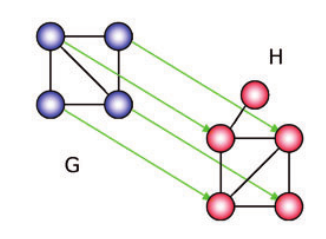
\includegraphics[height=0.25\textheight]{pic/measure.png}
\captionsetup{margin=50pt}
\caption{$G$为源网络,$H$为目标网络,其中各项指标的值分别为$EC=4/5=0.8,ICS=4/5=0.8,TWEC=0.8,S^3=4/6=0.67$ \cite{saraph2014magna} \label{fig:measure}}
\end{figure}

%@@@@@@@@@@@@@@@@@@@@@@@@@@@@@@@@@@@
\section{相关工作介绍}
关于PPI网络的全局匹配算法,到目前为止非常的多,本文主要对其中四种经典的算法进行简单的介绍。
%@@@@@@@@@@@@@@@@@@@@@@@@@@@@@@@@@@@@@@@@
\subsection{IsoRank算法}
IsoRank是全局网络匹配问题中被提出的第一个具有开拓性意义的算法。它主要分为两步。
第一步,IsoRank算法计算源网络$G_1$和目标网络$G_2$之间任意点对之间的相似性,用一个分数$R_{ij},i\in V_1,j\in V_2$来表示。IsoRank算法借鉴了Google的PageRank算法,任意点对$(i,j)$之间的价值由$i$和$j$两个点的邻居节点的价值所决定。

\begin{equation}\label{isorank1}
R=\sum R_{ij}=\sum_{u\in N(i),v\in N(j)}\frac{1}{\left | N(u) \right |\left | N(v) \right |}R_{uv}
\end{equation}
$N(i),N(j)$分别对应点i和点j的邻居点集。定义

\begin{equation}\label{isorank2}
A[i,j][u,v]=\begin{cases}
\frac{1}{\left | N(u) \right |\left | N(v) \right |} & \text{  } (i,u)\in E_1, (j,v)\in E_2 \\ 
 0& \text{  } \text{其他}
\end{cases}
\end{equation}
则有
\begin{equation}\label{isorank3}
R=AR
\end{equation}
从\ref{isorank3}可以看出,$R$是关于矩阵$A$的一个特征向量,在$A$是个稀疏矩阵的情况下,求解$A$的特征向量可以通过一种叫幂法(power method)的方法来迭代算出$R$,具体过程为:先随意初始化$R$,然后不断迭代,假设第$k$轮已经迭代完成,现在要进行第$k+1$轮迭代,则
\begin{equation}\label{isorank3}
R(k+1)\leftarrow AR(k)/\left \|AR(k)\right \|
\end{equation}
当$\left \|R(k+1)-R(k)\right \|\rightarrow 0$时即可终止迭代。
有了$R$,IsoRank第二步就是不断按分数从大到小挑选点对$(i,j)$,如果当前$i$和$j$都没有被匹配过,则将点对$(i,j)$加入最终的匹配结果,直到不能挑出符合条件的点对。
IsoRank可以说是全局网络匹配中第一个经典的算法,其经典之处在于其两步走的解决问题的方法。第一步定义点对之间的相似度,第二步根据相似度按某种策略产生匹配,这一解决问题的框架为之后不少提出的全局网络匹配算法所采用。
%@@@@@@@@@@@@@@@@@@@@@@@@@@@@@@@@@@@@@@@@@@@@@@@@@@@
\subsection{GRAAL算法}
GRAAL算法(GRAph ALigner)是一系列算法的总称,第一个提出的算法为GRAAL\cite{kuchaiev2010topological},而最近刚提出的算法为L-GRAAL\cite{malod2015graal}。这一系列算法的特征是都运用了一种叫小图度数(graphlet degree)的特征作为网络中一个点的拓扑结构的衡量标准。一个度数为$n$的小图(graphlet)就是一个有$n$个点的连通图(connected graph)。

图\ref{fig:graphlet}展示了所有点数在5以内的小图,可以看到这些小图的某些点被标了号,这些被标号的点被称为orbit,它们是小图中互相不同构的点。而对图$G$中的一个点$v$,其所谓的节点小图度数,是一个向量,其中向量的第$i$维表示的值就是以点$v$为中心,第$i$个orbit代表的小图出现的次数,形象化理解,就是将点$v$与第$i$个orbit匹配,看第$i$个orbit所在的小图是否能够匹配上以点$v$为中心延伸出去的子图,不同的子图分别计数,总出现次数就是第$i$维所表示的值。


\begin{figure}[htbp]
\centering
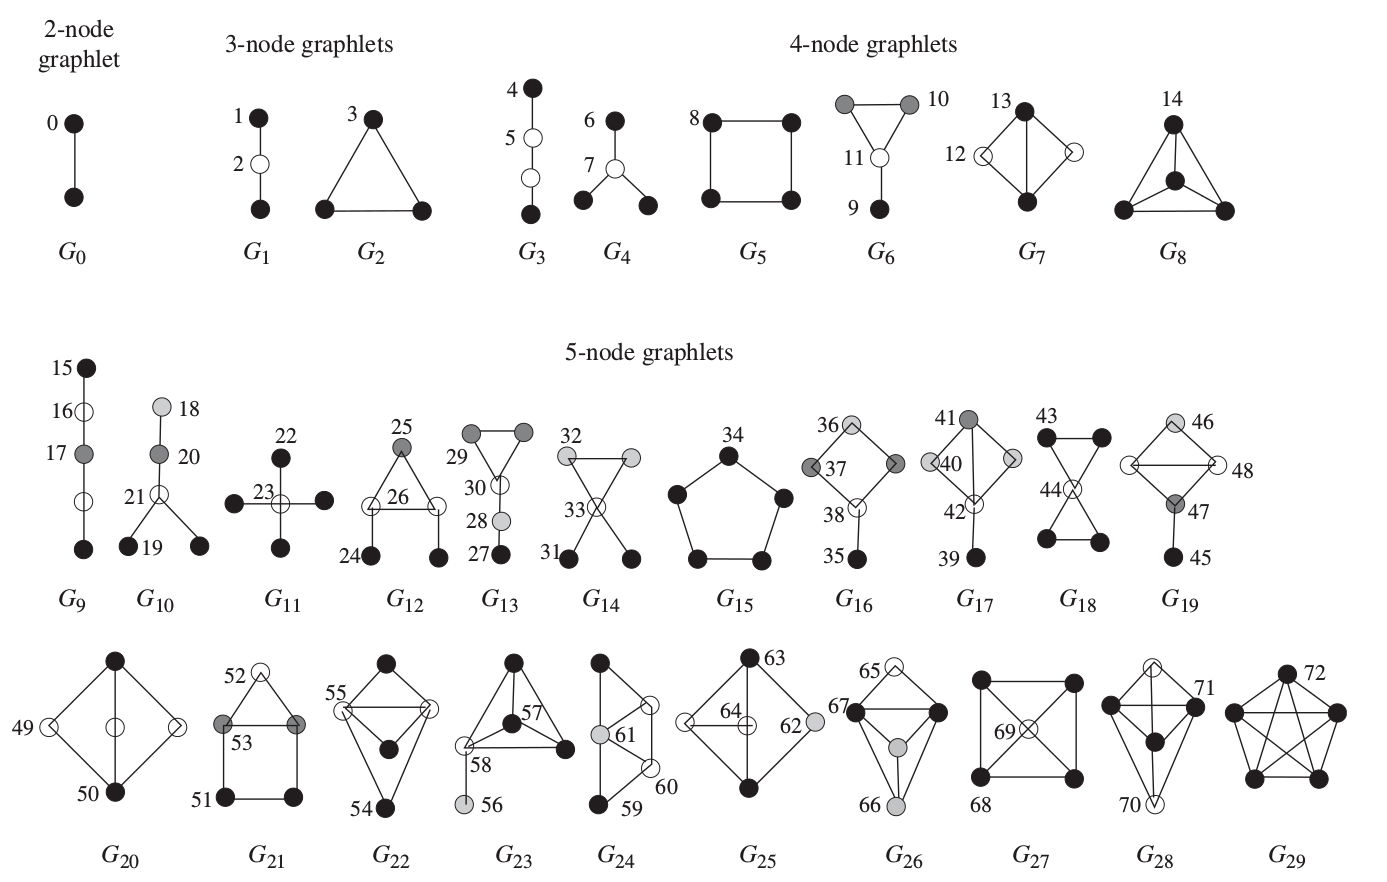
\includegraphics[width=\textwidth]{pic/graphlet.png}
\captionsetup{margin=50pt}
\caption{所有点数小于等于5的互不同构的小图\cite{kuchaiev2010topological}}\label{fig:graphlet}
\end{figure}

\begin{figure}[htbp]
\centering
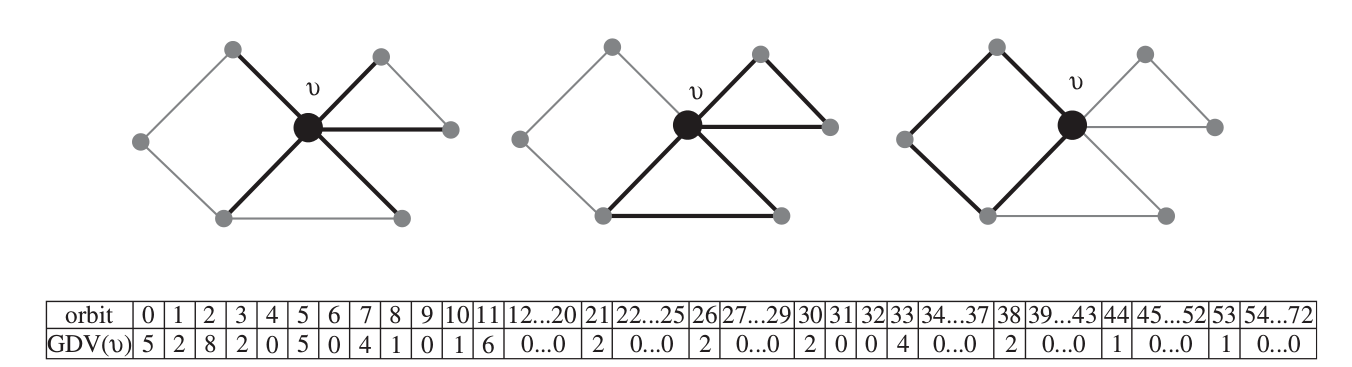
\includegraphics[width=\textwidth]{pic/orbitcount.png}
\captionsetup{margin=50pt}
\caption{点$v$的小图度数$GDV(v)\cite{kuchaiev2010topological}$}\label{fig:orbitcount}
\end{figure}

在由于小图度数这个衡量指标以后,类似于IsoRank,GRAAL也定义了两个点之间的相似度
\begin{equation}\label{graal1}
S(u,v)=1-\frac{\sum_{i=0}^{72}D_i(u,v)}{\sum_{i=0}^{72}w_i}
\end{equation}
其中
\begin{equation}\label{graal1}
D_i(u,v)=\frac{w_i*\left | log(u_i+1)-log(v_i+1) \right |}{log(max\{u_i,v_i\}+2)}
\end{equation}
$u_i$和$v_i$分别是点$u$和点$v$的第$i$维向量值,$w_i$是和第$i$个orbit相关的一个权重。

在有了相似度函数以后,GRAAL也和IsoRank一样,通过相似度函数,设计了一种寻找匹配的策略,然而不同于IsoRank的策略,GRALL采取的策略是,每次挑选出一个还没匹配过的点对$(i,j)$,称为种子点对(seed pair),然后将i的邻居点集和j的邻居点集根据相似度进行贪心的匹配,当i和j的邻居都不可再匹配的时候,GRAAL才继续寻找下一个种子点对,这是和IsoRank不同的地方。
GRAAL系列之后又出现了H-GRAAL\cite{milenkovic2010optimal},MI-GRAAL\cite{kuchaiev2011integrative},C-GRAAL\cite{memivsevic2012c}和L-GRAAL\cite{malod2015graal}。而最近提出的L-GRAAL\cite{malod2015graal}算法,通过解线性规划的问题来进行匹配,显示出了极好的匹配效果。

%@@@@@@@@@@@@@@@@@@@@@@@@@@@@@@@@@@@@@@@@@@@@@@@@@@@@@@@@@@@@@@@@@@@@@@
\subsection{SPINAL算法}
SPINAL算法(scalable protein interaction network alignment)也是类似于IsoRank和GRAAL的分两步算法。第一步,定义节点之间的相似度$P_{ij}$,并且与IsoRank类似的,它采用不断迭代的方式不断更新$P$的值,$P$的初始值由两个节点之间的度数差决定

\begin{equation}\label{spinal1}
P(i,j)=DegDiff(i,j)
\end{equation}

定义$NBG(\left \{ \left \langle i,j \right \rangle \right \},P)$为一个二分图,其中二分图左边的顶点集合由点$i$的邻居集合$N(i)$构成,右边的顶点集合由点$j$的邻居集合$N(j)$构成,边权则是它们对应的$P$值。
每一轮迭代,对于任意点对$(i,j)$,SPINAL算法对$NBG(\left \{ \left \langle i,j \right \rangle \right \},P)$进行二分图最大权匹配,令得到的匹配边集合为$C$,称为贡献者集合(contributors set),则新的$P$值为

\begin{equation}\label{spinal2}
P(i,j)=\frac{\sum_{(x_i,y_j)\in C}\frac{P(x_i,y_j)}{deg(x_i)*deg(y_j)}}{\sqrt{\left | C \right |}}
\end{equation}
通过若干论迭代,得到最后的相似度矩阵$P$。

SPINAL算法的第二步也是根据$P$矩阵对点对进行匹配的过程,和GRAAL算法类似,每一次,算法先找出当前$P$值最大的还未得到匹配的种子点对$(i,j)$,然后构造出由$i,j$的邻居集合构成的二分图,求出二分图的最大权值匹配边集合$M$。之后,SPINAL会重新依次检查二分图中的每一条非匹配边(不在集合$M$中),看看是否能够通过交换这条非匹配边与$M$中的匹配边得到更优的匹配。这相当于是一个局部调优的过程。然后再去寻找新的种子点对,进行下一轮的局部调优过程。
%@@@@@@@@@@@@@@@@@@@@@@@@@@@@@@@@@@@@@@@@@@@@@@@@@@@@@@@@@@@@@@@@@@@@
\subsection{PROPER算法}
PROPER算法(PROtein-protein interaction network alignment based on PERcolatin)\cite{kazemi2016proper}是一种基于图渗透的全局匹配算法。对于两个待匹配的图,PROPER算法用点对间的BLAST分数\cite{altschul1990basic}(一种衡量蛋白质序列之间相似度的分数)作为两个图任意点对之间的相似度函数

\begin{equation}\label{proper1}
S(i,j)=BLAST\_SCORE(i,j)
\end{equation}

与其他算法不同的是,在计算相似度的时候,PROPER算法并没有考虑点对之间的网络拓扑结构相似度,而只是单纯用了蛋白质序列的相似度。算法本身也是分两步走,第一步,算法按照相似度从大到小对所有点对进行排序。然后依次考虑每一点对$S(i,j)\geq l$,直到找到i和j都没有被匹配过的点对,将$(i,j)$加入集合$A$。最后的集合$A$就是第一步产生的部分匹配结果。

PROPER算法的第二步是在第一步结果$A$的基础上,扩展匹配的过程(图渗透算法)。定义

\begin{equation}\label{proper2}
F_A(i,j)=\left | \{(u,v):u\in N(i),v\in N(j),(u,v)\in A\} \right |
\end{equation}
称为点对$(i,j)$在已有匹配$A$下的贡献值,可以看到该值的实际意义就是,源网络在已有匹配$A$的情况下,通过匹配点对$(i,j)$能够增加的被匹配的边数。而匹配的衡量标准告诉我们被匹配的边数越多,则说明该匹配更好。因此,PROPER算法的第二步,便是将所有$F_A\geq r$且没有被匹配过的点对,按照$F_A$的值进行排序,挑选其中最好的一对加入集合$A$的过程。在集合$A$变化了以后,所有点对的$F_A$值重新计算,重新排序,重新挑选。

可以看到阈值$l$和$r$对PROPER算法有着极为重要的意义和影响。阈值$l$越小,第一步中被加入$A$的点对就越多,而阈值$r$越大,第二部中能够增加匹配的点对就越少。因此$l$和$r$分别控制了蛋白质序列相似度和网络结构相似度对整个算法的影响比例。

%@@@@@@@@@@@@@@@@@@@@@@@@@@@@@@@@@@@@@@@@@@@@@@@@@@@@@@@@@@@@@@@@@@@
\subsection{动态PPI网络生成}
本来,所有的PPI网络数据都是静态的,如何将PPI网络构造成动态的呢?\cite{zhang2016method}给出了一种合理的动态PPI网络构造方法。

基因表达数据(gene expression data)是对一个蛋白质在生物细胞作用中表现出来的基因水平提供衡量指标的数据。通过基因表达数据,我们可以很容易的直到生物体中的每一个蛋白质,在细胞生命活动的各个阶段,所表现出来的基因表达水平(gene expression level)分别是多少,可以知道,当蛋白质完成它在细胞活动中的作用是,其基因表达水平会明显下降,反之,则会处于高度活跃状态。因此,一个简单的想法就是,通过查看一个蛋白质的各个时刻的基因表达水平,来判断它在哪些时刻是处于活跃状态,那些时刻是处于不活跃状态的。定义一个蛋白质的基因表达数据为

\begin{equation}\label{dppi1}
p=[ p_1,p_2,p_3,....,p_n]
\end{equation}
$p$是一个数值序列,其中$p_i$为该蛋白质在$i$时刻的基因表达水平。\cite{zhang2016method}使用了一种三-西格玛阈值的方法来确定一个蛋白质何时处于活跃阶段,何时处于不活跃阶段。定义

\begin{equation}\label{dppi2}
Thresh_k(p)=\alpha (p)+k*\sigma (p)*\left (1-\frac{1}{1+\sigma ^2(p)}\right )
\end{equation}
为该蛋白质基因表达数据的三-西格玛阈值($k=1,2,3$)。其中$\alpha (p)$为$p$序列的平均值,$\sigma (p)$为标准差。

如果把$p$序列看成一个服从正态分布$N(\alpha,\sigma)$的随机变量,那么可以知道,$P(|X-\alpha|<\sigma)\approx 0.6827,P(|X-\alpha|<2\sigma)\approx 0.9545,P(|X-\alpha|<3\sigma)\approx 0.9973$。定义

\begin{equation}\label{dppi3}
Pr_i(p)= \begin{cases}
0.99 & \text{  } p_i\geq Thresh_3(p)\\ 
0.95 & \text{  } Thresh_3(p)> p_i\geq Thresh_2(p) \\ 
0.68 & \text{  } Thresh_2(p)> p_i\geq Thresh_1(p) \\ 
0 & \text{  } p_i<Thresh_1(p) 
\end{cases}
\end{equation}


为蛋白质在$i$时刻活跃的概率。那么

\begin{equation}\label{dppi4}
Pr_i((u,v))= Pr_i(u)*Pr_i(v)
\end{equation}
就是边$(u,v)$在$i$时刻活跃的概率。这样,一个静态的PPI网络就变成了由$n$个静态网络组成的动态PPI网络,其中每个蛋白质及蛋白质相互之间的作用在每个网络中都不同。
\renewcommand{\algorithmicrequire}{\textbf{Input:}}
\renewcommand{\algorithmicensure}{\textbf{Output:}}
\rhead{基于线段树优化的动态PPI网络匹配}
\chapter{基于线段树优化的动态PPI网络匹配}
%@@@@@@@@@@@@@@@@@@@@@@@@@@@@@@@@@@@@@@@@@@@@@
\section{动态PPI网络及动态PPI网络匹配}
由于本文要研究的问题是如何在动态PPI网络上作网络匹配,因此要先对动态PPI网络以及动态PPI网络匹配问题重新做出定义。

%@@@@@@@@@@@@@@@@@@@@@@@@@@@@@@@@@@@@@@@@@@@@@
\subsection{动态PPI网络定义}
一个动态PPI网络定义为四元组$G=(V,E,L,R)$,其中$V$是点集,$E$是边集,对于边集中的每一条边表示为$(u,v)$,其中$u$和$v$是在某一时刻具有相互作用的蛋白质点对。$L(u,v)$为边$(u,v)$处于活跃状态的开始时刻,$R(u,v)$为边$(u,v)$处于活跃状态的结束时刻,定义

\begin{equation}\label{myworkactivedefine}
Act_i(u,v)=\begin{cases}
1 & \text{  } L(u,v)\leq i\leq R(u,v), (u,v)\in E_2\\ 
0 & \text{  其他}  
\end{cases}
\end{equation}

用来表示边$(u,v)$在$i$时刻是否处于活跃状态。定义$Act_i(E)=\{(u,v):(u,v)\in E,Act_i(u,v)=1\}$表示$i$时刻下边集E中活跃的边组成的集合。

直观上看,一个动态PPI网络,就是在对应的静态PPI网络的基础上,加入了时间的元素,即每一条边$(u,v)$只会存在与某个连续的时间段$[L(u,v),R(u,v)]$内,而不是一直处于活跃状态。值得注意的是,在\cite{zhang2016method}中,动态PPI网络的定义与本文的定义稍有不同,本文为了简化问题,将边的活跃从原来的概率模型,转化成了0-1模型(即某一时刻,边$(u,v)$要么活跃,要么不活跃),并且假设每条边的活跃范围是一个连续的时间区间。对于多个时间区间的动态PPI网络定义也是可以的,本文的算法在这种情况下也是可以扩展的,简单起见,本文定义的时间区间个数限制在1个。

%@@@@@@@@@@@@@@@@@@@@@@@@@@@@@@@@@@@@@@@@@@@
\subsection{动态PPI网络构造}
本文主要用了\cite{zhang2016method}中的三-西格玛阈值方法,对静态PPI网络进行了动态化的转化,并且假设当边处于活跃状态的概率大于$0.5$时,边就是处于活跃状态的,否则就是不活跃状态。详细的动态PPI网络构造方法可以参见相关工作。

%@@@@@@@@@@@@@@@@@@@@@@@@@@@@@@@@@@@@@@@@@@
\subsection{动态PPI网络匹配}
本文研究的问题主要是一个静态PPI网络与一个动态PPI网络的匹配,两个动态PPI网络之间的匹配留作未来的研究工作。

有一个静态PPI网络$G_1=(V_1,E_1)$和一个动态PPI网络$G_2=(V_2,E_2,L,R)$,$|V_1|\leq |V_2|$定义动态PPI匹配$f:V_1\rightarrow V_2$为点集$V1$到点集$V2$的一个单射。

在源网络$G_1$中,如果边$(u,v)$在时刻$i$满足$Act_i(f(u),f(v))=1$,则称边$(u,v)$在时刻$i$是被保留(匹配)的。

定义$f_i(E_1)=|\{(u,v):(u,v)\in E_1, \text{且} (u,v)\text{在$i$时刻是被保留的}\}|$为源网络边集$E_1$在$i$时刻被保留的边的集合。

在动态PPI网络的环境下,所有的匹配衡量标准都需要重新定义,我们称这些衡量标准为动态匹配衡量标准(dynamic alignment quality measure)。分别有
\begin{equation}\label{myworkecdefine}
    EC(f)=\underset{i}{max}\frac{\left | f_i(E_1) \right |}{\left | E_1 \right |}
\end{equation}
\begin{equation}\label{myworkicsdefine}
    ICS(f)=\underset{i}{max}\frac{\left | f_i(E_1) \right |}{\left |Act_i(E_2(G_2[f(V_1)]))\right |}
\end{equation}
\begin{equation}\label{myworks3define}
S^{3}(f)=\underset{i}{max}\frac{\left | f_i(E_1) \right |}{\left | E_1 \right |+\left |Act_i(E_2(G_2[f(V_1)])) \right |-\left | f_i(E_1) \right |}
\end{equation}
\begin{equation}\label{myworktwecdefine}
    TWEC(f)=\frac{EC(f)+ICS(f)}{2}
\end{equation}
可以看到,在动态PPI网络的环境下,所有的衡量标准,都得到了动态化的定义,其本质,就是在匹配$f$下,将动态PPI网络看成若干个静态网络后,将源网络与这些静态网络逐个进行匹配结果衡量,最终选取值最大的结果。

有了动态匹配衡量标准的定义,对于本文研究的问题,便是找到一个匹配$f$使得动态匹配衡量标准最大化,即
\begin{equation}\label{myworktwobjdefine}
    objf=\underset{f}{argmax}Q(f)
\end{equation}
其中的$Q$可以是上述衡量标准的任意一项。针对$objf$,是否可以用已有的静态网络匹配算法来寻找呢?

%@@@@@@@@@@@@@@@@@@@@@@@@@@@@@@@@@@@@@@@@@@@@@@@@@@
\section{静态匹配算法的缺陷}
根据新的动态PPI网络匹配定义以及衡量匹配的标准,是否可以将已有的静态网络匹配算法应用到动态PPI网络匹配这个问题上呢?答案是肯定的,但是缺点就是时间或者匹配效果的下降。

第一种方案是,单纯忽略$L$和$R$的信息,将$G_2(V_2,E_2,L,R)$转化成对应的静态PPI网络$G_2(V_2,E_2)$,然后利用静态PPI网络匹配算法去算得匹配$f$,当做最后的结果$objf$。但是这样做的问题在于,直接把动态PPI网络的一条边当做静态网络边,意味着这条边在所有时刻都是活跃的,但是实际上这条边只在某些时刻才是处于活跃状态的,因此既有的匹配算法无论在相似度的估计上,还是匹配生成上,都会被这条看似永久活跃,其实只在某些时候活跃的边所“迷惑”,产生不精准的相似度估计或者匹配方案。

第二种方案,便是将动态PPI网络$G_2$拆分成若干张静态PPI网络,然后逐个进行匹配,从中选取拥有最好匹配效果的匹配方案。这种方法的好处在于,匹配算法确实是跑在了真实的网络上,但是缺点在于时间,假设动态PPI网络的时间跨度非常大,那么这种方法会让匹配算法非常耗时(从本来的只要匹配一次变成匹配$N$次),这对于一些已经比较耗时的匹配算法来说,无疑是不可接受的。

因此,我们希望得到一个不但时间消耗不大,且依旧能够得到较优匹配效果的算法。为此,本文提出了SGOPT(SeGment tree OPTimization)算法,不仅能够在既有静态匹配算法的基础上提高匹配效果,时间上也不会像逐个匹配一般地耗时,可以说是一种折中的算法,最关键的是,它是基于动态PPI网络所提出的算法,不同于已有的静态匹配算法,是对动态PPI网络这个新环境下的新问题的一种创新性的尝试。
%@@@@@@@@@@@@@@@@@@@@@@@@@@@@@@@@@@@@@@@@@@@@
\section{SGOPT算法}
这一部分主要介绍SGOPT算法,也是本文主要工作所在。可以看到,在所有动态匹配衡量标准的定义中,分子都是$|f_i(E_1)|$,而这个分子的意义,就是在$i$时刻,源网络$G_1$在通过匹配$f$的情况下,$E_1$中仍然被保留(匹配)的边的集合。一个直观的想法,就是不断调整匹配$f$,使得

\begin{equation}\label{myworkmaxfidefine}    
\underset{i}{max}\{ |f_i(E_1)|\}
\end{equation}

最大化。而要计算公式\ref{myworkmaxfidefine}的值,需要考查每一时刻$i$下,$E_1$中被保留的边数,假设时间跨度为$T$,则需要$\mathcal{O}(|E_1|*T)$的时间才能完成。SGOPT算法做的第一步,就是将这个时间从$\mathcal{O}(|E_1|*T)$变成了$\mathcal{O}(|E_1|*log(T))$,也就是说,对于$E_1$中的一条边,计算它在所有时刻内是否被保留,从原本的时间复杂度$\mathcal{O}(T)$,变成了$\mathcal{O}(log(T))$。

SGOPT算法的第二步,则是在第一步时间优化的基础上,通过一种局部调整的策略,逐步匹配$f$,使得公式\ref{myworkmaxfidefine}最大化。

SGOPT算法的第一步,从时间上优化了计算匹配衡量标准的计算耗时,第二步则是从第一步的基础上,使得对动态PPI网络的匹配,可以从逐个匹配的劣势下,变为只对一个网络进行匹配。

%@@@@@@@@@@@@@@@@@@@@@@@@@@@@@@@@@@@@@@@@@@@@@@@
\subsection{从$\mathcal{O}(T)$到$\mathcal{O}(log(T))$的转化}
先考虑这样一个问题,假设有一个整数序列,长度为$T$,序列为

\begin{equation}\label{myworkseqdefine}    
[a_1,a_2,a_3,.....,a_T]
\end{equation}

其中$a_i$为序列中第$i$个整数。现在有三种操作。

第一种,把第$l$个到第$r$个($l\leq r$)的所有整数都加上一个共同的数字$d$,简称$ADD(l,r,d)$。

第二种,把第$l$个到第$r$个($l\leq r$)的所有整数都减去一个共同的数字$d$,简称$SUB(l,r,d)$。

第二种,求出第$l$个到第$r$个($l\leq r$)的所有整数中最大的那个数,简称$MAX(l,r)$。

那么如何快速地完成这些操作呢?答案是用线段树(segment tree)这种数据结构\cite{de2000computational}。线段树是一种非常适合维护区间上操作的数据结构,对于一个长度不超过$T$的区间,其本质是一颗高度不超过$\mathcal{O}(log(T))$满二叉树,线段树的空间复杂度为$\mathcal{O}(T)$,而对于上述的三种操作中的任意一种操作,线段树都能够在不超过树高$\mathcal{O}(log(T))$的时间复杂度内完成。

那么这个问题对于本文研究的问题有什么作用呢?答案是可以将计算公式\ref{myworkmaxfidefine}的过程转化成该问题,然后用线段树在$\mathcal{O}(log(T))$时间内解决。

考虑本文研究问题的一个部分匹配$fp$,不同于$f$的是,$G_1$中的点$v$在部分匹配$fp$下可能并没有对应的$G_2$中的匹配点,用$fp(v)=undefined$来表示。同时用$fp^{-1}(v)=undefined$来表示$G_2$中的点$v$并没有被$G_1$中的任何一个点所匹配。

假设在$fp$这个匹配下,我们已经知道了所有的$|fp_i(E_1)|$的值($fp_i(E_1)$即为在匹配fp的情况下,在$i$时刻时$E_1$中被保留的边的集合。),这样的值共有$T$个,构成了一个整数序列,定义为

\begin{equation}\label{myworkfseqdefine}    
SEQ(fp)=[|fp_1(E_1)|,|fp_2(E_1)|,.....,|fp_T(E_1)|]
\end{equation}

现在,我们需要往$fp$匹配中添加一对新的匹配$(u,v)(u\in V_1,v\in V_2,fp(u)=undefined,fp^{-1}(v)=undefined)$。且令新的匹配为$fn=fp\bigcup (u,v)$。定义

\begin{equation}\label{myworkfadddefine}    
SEQ(fn)=ADD\_MATCH(SEQ(fp),(u,v))
\end{equation}

来表示这样的一种加匹配$(u,v)$的操作,在$ADD\_MATCH$操作后,$SEQ(fp)$变成了$SEQ(fn)$。而$ADD\_MATCH$操作,就是将$fp$匹配下各个时刻的$E_1$保留的边数,变成了$fn$匹配下各个时刻的$E_1$保留的边数。

在添加了匹配$(u,v)$后,考查满足$x\in N(u),y\in N(v),fp(x)=y$的任意点对$(x,y)$。由定义可知,在$E_1$中,边$(u,x)$通过匹配$fn$被映射到了$E_2$中的$(v,y)$,而边$(v,y)$在$[L(v,y),R(v,y)]$这个时间区间内是处于活跃状态的,所以对于任意时刻$i\in [L(v,y),R(v,y)]$,$fn_i(E_1)$因为$(u,v)$匹配的加入,而在$fp_i(E_1)$的基础上,多了$(u,x)$这一条边。也就是说,$SEQ(fp)$这个序列在$[L(v,y),R(v,y)]$这个区间内的所有数值都加了1,这不就是对$SEQ(fp)$进行了ADD(L(v,y),R(v,y),1)操作么?

如果用一颗长度为$T$的线段树来维护$SEQ(fp)$,那么每次的$ADD\_MATCH$操作,都可以通过对该线段树进行若干次(由符合条件的u和v的邻居点对个数决定)$ADD$操作来实现从$SEQ(fp)$到$SEQ(fn)$的转化,因此,其时间复杂度就是$\mathcal{O}(log(T))$。而通过不断加匹配,从部分匹配变成单射的时候(即$G_1$中每个点都得到了匹配),这颗线段树所维护的,正是$SEQ(f)$,而$SEQ(f)$中的最大值,正是公式\ref{myworkmaxfidefine}所要求的值,可以通过对该线段树进行$MAX(1,T)$操作来得到。这样,我们就完成了从$\mathcal{O}(T)$到$\mathcal{O}(log(T))$的转化。

%@@@@@@@@@@@@@@@@@@@@@@@@@@@@@@@@@@@@@@@@@@@@@@@@@@
\subsection{局部调整策略}
在有了线段树这一利器后,我们已经做到了可以对任意部分匹配$fp$,随时维护$SEQ(fp)$,根据$ADD\_MATCH$操作,我们可以从一个空的匹配集合和一颗序列长度为$T$且数值全为0的线段树开始,不断加入新的匹配$(u,v)$,在$\mathcal{O}(log(T))$的时间内更新序列,直到再没有匹配能够加入为止,最终产生的结果就是全局匹配$f$。

因此,利用这个框架,SGOPT算法可以结合任意已有的静态PPI网络匹配算法,将它们的匹配$f$结果作为输入,可以在$\mathcal{O}(|E_1|*log(T))$时间内算出$SEQ(f)$,比之前$\mathcal{O}(|E_1|*T)$的方式快了很多。

而且,在这个框架下,我们不但可以加入匹配,也可以删除匹配,同样可以在$\mathcal{O}(log(T))$时间内维护$SEQ(fp)$,比原本$\mathcal{O}(T)$的时间快了许多。因此,在这个优化框架下,本文提出了一种能够在动态PPI网络环境下的局部调整策略,使得得到的匹配在公式\ref{myworkmaxfidefine}下最大化。

类似于$ADD\_MATCH$,定义$DEL\_MATCH(SEQ(fn),(u,v))$操作表示将匹配$(u,v),fp(u)=v$从匹配$fn$中删去,而得到的新的匹配为$fp=fn-{(u,v)}$。对于删除匹配$(u,v)$,考查满足$x\in N(u),y\in N(v),fn(x)=y$的任意点对$(x,y)$,进行$SUB(L(v,y),R(v,y),1)$操作,同样可以在$\mathcal{O}(log(T))$的时间复杂度内完成。

于是,对于一个匹配$fp$,无论是添加一对匹配$(u,v)$,还是删除一对匹配$(u,v)$,都可以在$\mathcal{O}(log(T))$内做到。

局部调整策略的伪代码可以见算法\ref{alg:1}。算法的总体思想是通过随机删除已有匹配的一部分,并且加入一部分别的匹配来调整当前匹配。

$\alpha$和$\beta$都是参数,分别表示迭代次数上限以及匹配删除比例。

第1行到第3行是初始化过程,对于任意匹配$f$,算法将该匹配$f$作为需要调整的初始匹配,用线段树来维护$SEQ$序列。$ADD\_MATCH(SEQ,f)$是一系列$ADD\_MATCH(SEQ,(u,v)),(u,v)\in f$操作的集合(下同)。

第5行到第20行是整个迭代的循环,迭代的次数有$\alpha$参数决定,整个循环是不断调整既有匹配集合$fp$的过程。

第6行到第11行,算法从$fp$中随机挑出若干个匹配,挑出的数目由参数$\beta$决定,并且把这些匹配从$fp$中用操作$DEL\_MATCH(SEQ,f\_delete)$删去。

第12行到第12行,算法构造了一个二分图$bg$,点集分别有$G_1$和$G_2$中未被匹配的点构成,而任意点对$(u,v)$直接间的权重,由函数$NS(fp,u,v)$决定。

\begin{equation}\label{myworknsdefine}
    NS(f,u,v)=|\{(x,y):x\in N(u),y\in N(v),f(x)=y\}|
\end{equation}
$NS(f,u,v)$的值本质上,就是在匹配$f$的情况下,如果加入匹配$(u,v)$,能够对$E_1$中保留的边数增加的一个数值的估计,直观上可以认为,$NS(f,u,v)$越大,匹配$(u,v)$的效果越好。

第13行到第19行,得到二分图$bg$的最大权重匹配,将对应的匹配加入得到新的$fp$,最后比较新的$fp$在调整前后的好坏,如果好于调整前的,则说明这轮迭代找到了一个更优的匹配,否则,进行下一轮的迭代。

值得说明的是,这个二分图的最大权重匹配,不包括权值为0的边(对既有匹配没有任何贡献效益),所以在这个调整过程中,会存在某些点没有得到匹配,所以这些点在下一轮迭代中,和会那些被删掉匹配的点放在一起,重新构建一个新的二分图。这就导致了该算法可能会出现的“换入换出”(swap-in,swap-out)效果。每一次迭代,算法会“换出”一部分匹配,同时,“换入”一部分之前被删掉的匹配。本文认为,这样的局部调整策略具有较好的效果。

此算法的时间复杂度为$\mathcal{O}(\alpha\beta log(T))$,和两个参数息息相关。过小的参数可能会导致匹配效果糟糕,过大的参数,则会导致算法非常耗时,因此,需要在两个参数之间作出权衡。

\begin{small}
\begin{algorithm}[!htb]
{
\caption{局部调整算法}
\label{alg:1}
    \begin{algorithmic}[1]
    \Require
    $G_1(V_1,E_1)$:源网络
    
    $G_2(V_2,E_2,L,R)$:目标网络
    
    $f$:当前匹配
    
    $\alpha$:参数$\alpha>0$
    
    $\beta$:参数$0<\beta<1$
    
    \Ensure
    $fp$: 新的匹配
    
    \State $fp \gets f$
    \State $SEQ \gets [0,0,...,0]$
    \State $SEQ \gets ADD\_MATCH(SEQ,f)$
    \State $iteration\_count \gets 0$
    \While{$iteration\_count<\alpha$}
        \State $iteration\_count\gets iteration\_count+1$
        \State $oldSEQ\gets oldSEQ$
        \State $oldfp\gets fp$
        \State $f\_delete\gets$从$fp$中随机挑选的$\beta*|V_1|$个匹配
        \State $SEQ\gets DEL\_MATCH(SEQ,f\_delete)$
        \State $fp \gets fp-f\_delete$
        \State $bg\gets WeightedBipartiteGraph(\{u:fp(u)=undefined\},\{v:fp^{-1}(v)=undefined\},NS(fp,u,v))$
        \State $M\gets MaximumWeightedBipartiteGraphMaching(bg)$
        \State $fp\gets fp\bigcup M$
        \State $SEQ\gets ADD\_MATCH(SEQ,M)$
        \If{$MAX(SEQ)<MAX(oldSEQ)$}
            \State $SEQ\gets oldSEQ$
            \State $fp\gets oldfp$
        \EndIf
    \EndWhile
    \end{algorithmic}    
}
\end{algorithm}
\end{small}



\rhead{实验与结果分析}
\chapter{实验与结果分析}

%@@@@@@@@@@@@@@@@@@@@@@@@@@@@
\section{数据集及预处理}
实验所用的所有数据均来自IsoBase数据库\cite{park2011isobase}。Isobase数据库是被普遍使用的生物PPI网络数据库,因此我们选择了这个数据集。该数据集包含了四种生物的PPI网络数据,分别是Saccharomyces cerevisiae(简写为S.cerevisiae或sc),Drosophila melanogaster(简写为D.melanogaster或dm),Caenorhabditis elegans(简写为C.elegans或ce)以及Homo sapiens(简写为H.sapiens或hs)。本文使用\cite{zhang2016method}的方法,构造了四个对应的动态PPI网络,并且实验所用的静态PPI网络是从对应的动态PPI网络中抽取的分时网络,而不是原PPI网络。对于抽取的分时网络,每种生物的网络详细信息见表\ref{table:1.1}。

\begin{table}[htbp]
    \centering
    \caption{实验所用的静态PPI网络(分时网络)}
    \label{table:1.1}
    \begin{tabular}{cccc}
         \hline 物种&点数&边数&平均点度\\
         \hline C.elegans&2974&2653&1.78\\
         D.melanogaster&7387&14004&3.79\\
         H.sapiens&10296&30349&5.90\\
         S.cerevisiae&5523&46207&16.73\\
         \hline
    \end{tabular}
\end{table}

而四个动态PPI网络的详细信息,见表\ref{table:1.2}。

\begin{table}[htbp]
    \centering
    \caption{实验所用的动态PPI网络}
    \label{table:1.2}
    \begin{tabular}{cccc}
         \hline 物种&T&点数&平均边数\\
         \hline C.elegans&15&2974&1896.87\\
         D.melanogaster&15&7387&9995.27\\
         H.sapiens&15&10296&21772.73\\
         S.cerevisiae&15&5523&32990.53\\
         \hline
    \end{tabular}
\end{table}

%@@@@@@@@@@@@@@@@@@@@@@@@@@@@@@@@@
\section{实验方法与环境}
本文使用了全局比对算法中的四种经典算法作为和本文算法的对比,分别是IsoRank\cite{singh2008global},SPINAL\cite{aladaug2013spinal},L-GRAAL\cite{malod2015graal}和PROPER\cite{kazemi2016proper}算法。SGOPT算法全部代码由Java构成,并且运行在Linux Ubuntu环境下,详细的环境参数见表\ref{table:2}。

对于这四种不同的静态比对算法,首先使用方案一和方案二产生两种不同的比对结果,其次,本文采用SGOPT在方案一产生的比对结果上进行优化,产生第三种比对结果,对比这三种情况下的比对结果的好坏程度。至于如何衡量比对结果的好坏,本文首先以CE指标和运行时间作为主要考量的指标,然后再比较本文中新定义的四个动态比对衡量指标,即DEC,DICS,DS$^3$和DTWC。

\begin{table}[htbp]
    \centering
    \caption{实验运行环境}
    \label{table:2}
    \begin{tabular}{l|l}
         \hline 
         CPU&Intel Core i7-4790K, 4.00GHz\\
         \hline
         内存&16G\\
         \hline
         操作系统&Linux Ubuntu 14.04LTS,64位\\
         \hline
    \end{tabular}
\end{table}

本文使用\textit{算法-方案一}和\textit{算法-方案二}来表示某种算法其在方案一下和方案二下产生的比对结果,而\textit{SGOPT-算法}表示某种算法在方案一下产生的结果经过SGOPT优化后得到的第三种比对结果。例如,\textit{IsoRank-方案一}就表示IsoRank算法在方案一下产生的比对结果,\textit{SGOPT-IsoRank}就表示SGOPT优化这个结果产生的新的比对结果。

为了简单起见,本文用\textit{生物1-生物2}来表示对\textit{生物1}的静态PPI网络与\textit{生物2}的动态PPI网络进行比对所得到的比对结果。例如\textit{ce-dm}表示将生物\textit{C.elegans}和\textit{D.melanogaster}进行比对得到的结果。

除了对比SGOPT与其他的静态比对算法,本文还测试了SGOPT算法的两个参数对SGOPT效果的影响。

%@@@@@@@@@@@@@@@@@@@@@@@@@@@@@@@@@@@@@
\section{$\alpha,\beta$参数对结果的影响}

\subsection{$\beta$参数的影响}
参数$\beta$影响的是每次删掉的匹配点对数,因此$\beta$越大,删掉的匹配点对数便越多,二分图便越大,导致一次迭代的时间就越长。图\ref{beta}是不同$\beta$情况下SGOPT算法的运行结果。从图\ref{beta1}中可以看到,对于一个固定的$\beta$,运行时间越长,则比对的效果越好。另一方面,在同样的运行时间下,越小的$\beta$有越好的效果,$\beta=600$时,SGOPT甚至不能提高初始比对结果的CE指标,这是因为当一轮迭代中删去的匹配点对过多的时候,SGOPT面对的是一个需要全局优化的局面,而SGOPT只适于局部优化的情况,所以在全局优化的情况下,SGOPT并不能很快找到一个拥有更高CE指标的比对结果。所以SGOPT适合$\beta$比较小的情况。

而图\ref{beta2}则是$\beta$比较小的时候,SGOPT算法的实验结果。可以看到此时,不同$\beta$下的结果并没有明显的差别。最终,本文设置$\beta=35$做为实验的默认参数。

\begin{figure}[htbp]
    \subfigure[$\beta$从50到2000变化时(步长50)的实验结果]{
        \begin{minipage}[b]{0.5\linewidth}
            \centering
            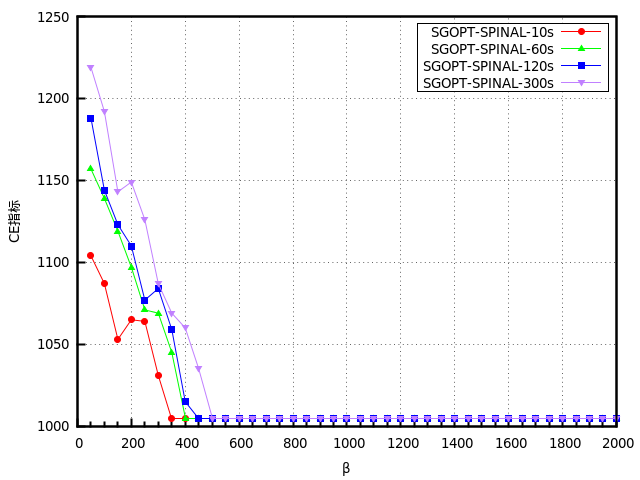
\includegraphics[width=\linewidth]{pic/beta1.png}
            \label{beta1}
        \end{minipage}
    }
   \subfigure[$\beta$从5到50变化时(步长3)的实验结果]{
        \begin{minipage}[b]{0.5\linewidth}
            \centering
            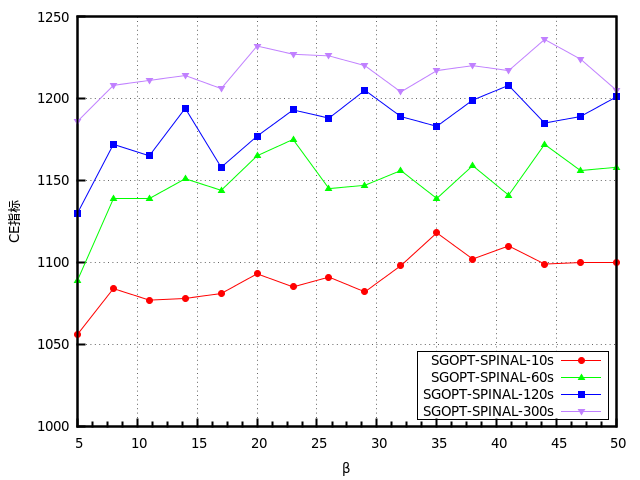
\includegraphics[width=\linewidth]{pic/beta2.png}
            \label{beta2}
        \end{minipage}
    }
    \caption{在\textit{ce-dm}实验组下,不同$\beta$值对\textit{SGOPT-SPINAL}的实验结果的影响。不同曲线代表不同的运行时间。 }
    \label{beta}
\end{figure}

%@@@@@@@@@@@@@@@@@@@@@@@@@@@@@@@@@@@@@@@@@@@@@@@@@@
\subsection{$\alpha$参数的影响}

$\alpha$参数控制SGOPT算法的迭代轮数,从SGOPT算法可以看出,随着迭代论次的不断变化,比对的CE指标会不断得到提高,可以从图\ref{alpha}中看出来。为了进一步考察迭代轮数对算法结果的影响,参见图\ref{alphad},从中可以看出,随着迭代轮次的加多,CE指标得到提高的机会越来越少,说明算法有个收敛的过程,虽然理论上,随着迭代次数的增加,CE指标会越来越高,但是考虑到运行时间的关系,本文最终设置$\alpha=15000$作为实验的默认参数。

\begin{figure}[htbp]
    \subfigure[CE指标随迭代论次变化的结果]{
        \begin{minipage}[b]{0.5\linewidth}
            \centering
            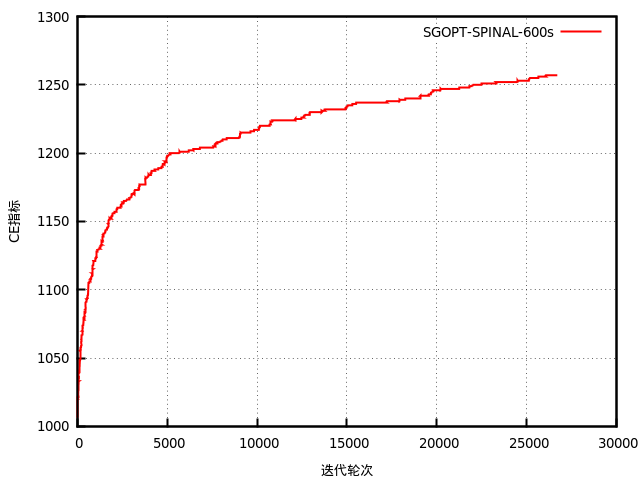
\includegraphics[width=\linewidth]{pic/alpha.png}
            \label{alpha}
        \end{minipage}
    }
   \subfigure[CE指标(差值)随迭代论次变化的结果]{
        \begin{minipage}[b]{0.5\linewidth}
            \centering
            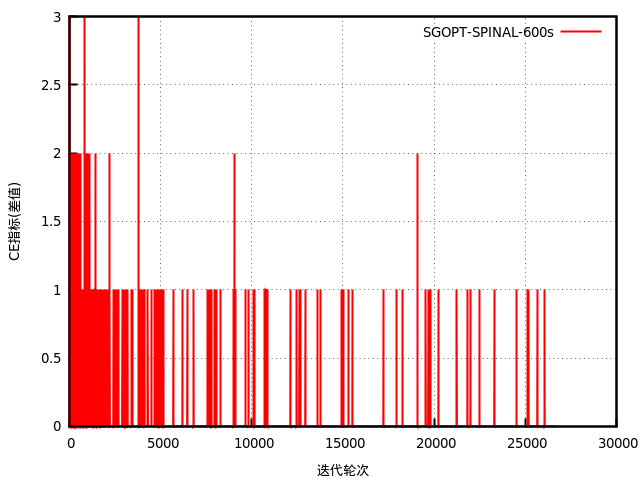
\includegraphics[width=\linewidth]{pic/alphad.png}
            \label{alphad}
        \end{minipage}
    }
    \caption{在\textit{ce-dm}实验组下,\textit{SGOPT-SPINAL}的CE指标随迭代论次增加而变化的实验结果。}
    \label{alphaall}
\end{figure}


%@@@@@@@@@@@@@@@@@@@@@@@@@@@@@@@@@@@@@@@@@
\section{不同算法之间的比较}

对于实验中要比较的四种静态算法,本文使用它们的默认参数,见表\ref{table:3}。

\begin{table}[htbp]
    \centering
    \caption{静态比对算法与运行参数}
    \label{table:3}
    \begin{tabular}{ccc}
         \hline 算法&命令行&参数\\
         \hline IsoRank&-alpha $\alpha$ -I 50&$\alpha=1$\\
         SPINAL&-II -alpha $\alpha$&$\alpha=1$\\
         L-GRAAL&-alpha $\alpha$&$\alpha=1$\\
         PROPER&$-l$ $l$ $-r$ $r$&$l=500,r=1$\\
         \hline
    \end{tabular}
\end{table}

%@@@@@@@@@@@@@@@@@@@@@@@@@@@@@@@@@@@@
\subsection{CE指标与运行时间}
图\ref{ce-dm}是\textit{ce-dm}实验组的结果。图\ref{ce-dm-CE}是CE指标的实验结果,图\ref{ce-dm-Time}则是运行时间的结果。从CE指标来看,SGOPT算法好于方案一,差于方案二,唯一的例外是对于IsoRank这个算法,SGOPT的优化效果远远超出了预期。从运行时间上来看,SGOPT的运行时间与方案一相比,只多了其调整比对所运行的时间。对于方案二,由于需要对静态网络和每个分时网络逐一进行比对,整个过程十分耗时。综合考虑,SGOPT在效果上比方案一好,在时间上远快于方案二,不失为一种折中的方案。

\begin{figure}[htbp]
    \subfigure[CE指标]{
        \begin{minipage}[b]{0.5\linewidth}
            \centering
            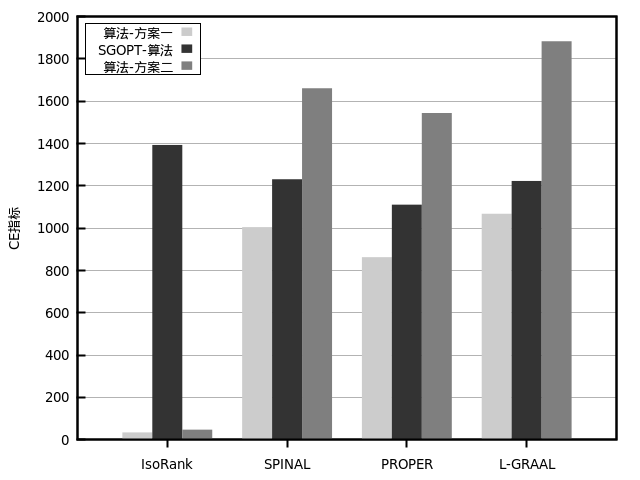
\includegraphics[width=\linewidth]{pic/ce-dm-CE.png}
            \label{ce-dm-CE}
        \end{minipage}
    }
   \subfigure[运行时间]{
        \begin{minipage}[b]{0.5\linewidth}
            \centering
            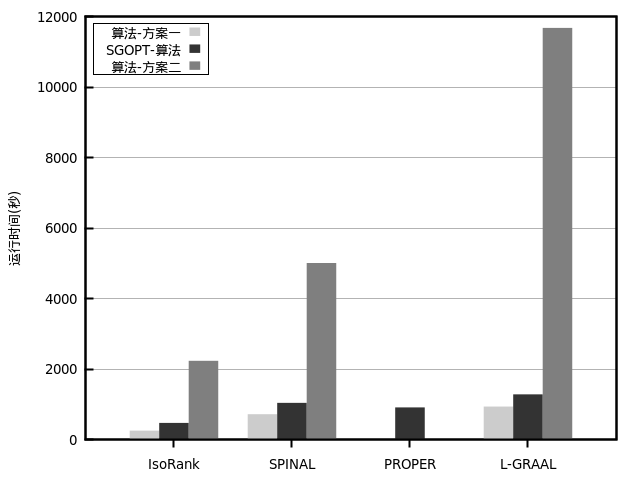
\includegraphics[width=\linewidth]{pic/ce-dm-Time.png}
            \label{ce-dm-Time}
        \end{minipage}
    }
    \caption{在\textit{ce-dm}实验组下,四种静态算法在三种方案下的实验结果。}
    \label{ce-dm}
\end{figure}

对于剩下的实验组,结果可见图\ref{ce-hs},\ref{ce-sc},\ref{dm-hs},\ref{dm-sc},\ref{hs-sc}。可以看到结果是类似的。在\textit{hs-sc}实验组中,SGOPT对SPINAL的优化效果,甚至好于SPINAL在方案二下的结果。

值得一提的是PROPER算法,从实验中可以看到PROPER算法无论从时间上还是CE指标上,都是好于SGOPT的。但是值得注意的是在本实验中$T=15$,对于SGOPT算法来说很难凸显它的优势,因为实际情况中的动态PPI网络都是时间跨度比较小的网络。但是本文的算法同样适用于除PPI网络比对之外的其他的网络比对问题,在T较大的情况下,SGOPT算法的时间优势才得以体现。

\begin{figure}[htbp]
    \subfigure[CE指标]{
        \begin{minipage}[b]{0.5\linewidth}
            \centering
            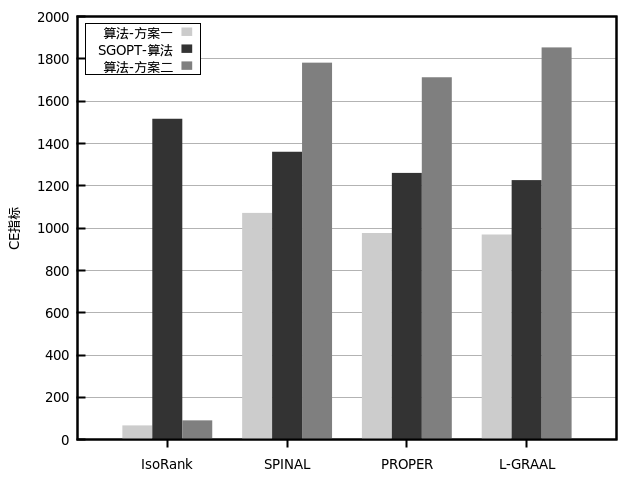
\includegraphics[width=\linewidth]{pic/ce-hs-CE.png}
            \label{ce-hs-CE}
        \end{minipage}
    }
   \subfigure[运行时间]{
        \begin{minipage}[b]{0.5\linewidth}
            \centering
            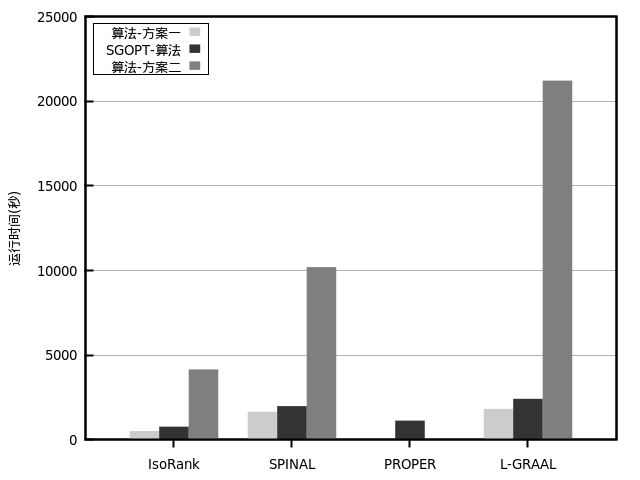
\includegraphics[width=\linewidth]{pic/ce-hs-Time.png}
            \label{ce-hs-Time}
        \end{minipage}
    }
    \caption{在\textit{ce-hs}实验组下,四种静态算法在三种方案下的实验结果。}
    \label{ce-hs}
\end{figure}


\begin{figure}[htbp]
    \subfigure[CE指标]{
        \begin{minipage}[b]{0.5\linewidth}
            \centering
            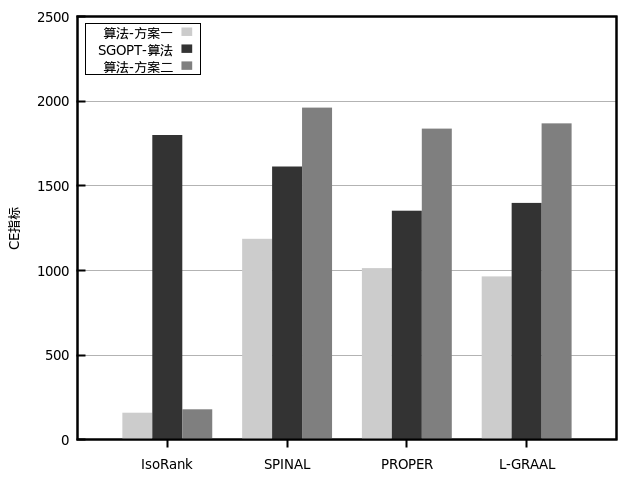
\includegraphics[width=\linewidth]{pic/ce-sc-CE.png}
            \label{ce-sc-CE}
        \end{minipage}
    }
   \subfigure[运行时间]{
        \begin{minipage}[b]{0.5\linewidth}
            \centering
            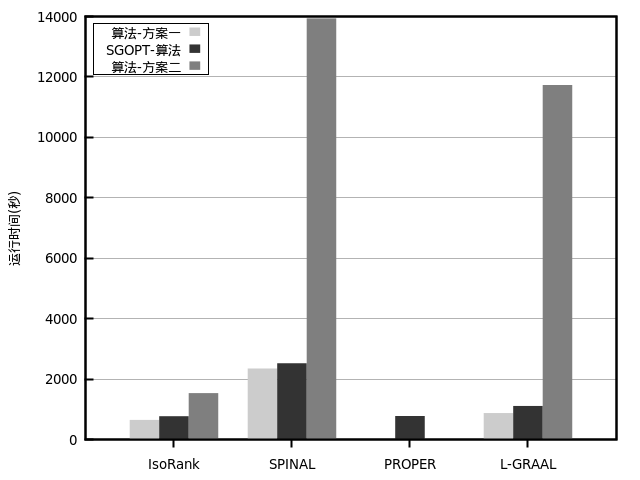
\includegraphics[width=\linewidth]{pic/ce-sc-Time.png}
            \label{ce-sc-Time}
        \end{minipage}
    }
    \caption{在\textit{ce-sc}实验组下,四种静态算法在三种方案下的实验结果。}
    \label{ce-sc}
\end{figure}

\begin{figure}[htbp]
    \subfigure[CE指标]{
        \begin{minipage}[b]{0.5\linewidth}
            \centering
            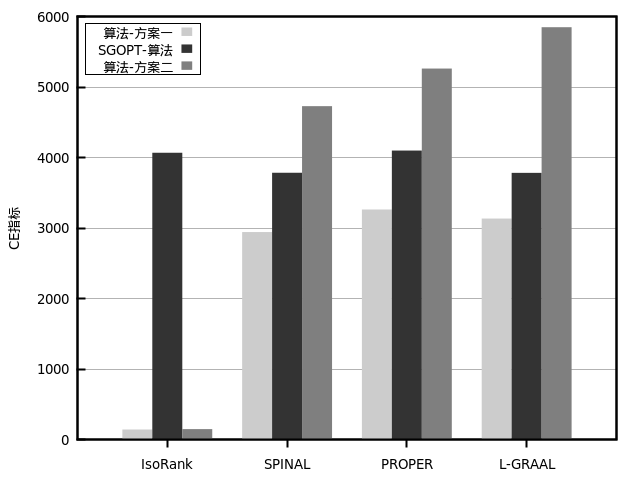
\includegraphics[width=\linewidth]{pic/dm-hs-CE.png}
            \label{dm-hs-CE}
        \end{minipage}
    }
   \subfigure[运行时间]{
        \begin{minipage}[b]{0.5\linewidth}
            \centering
            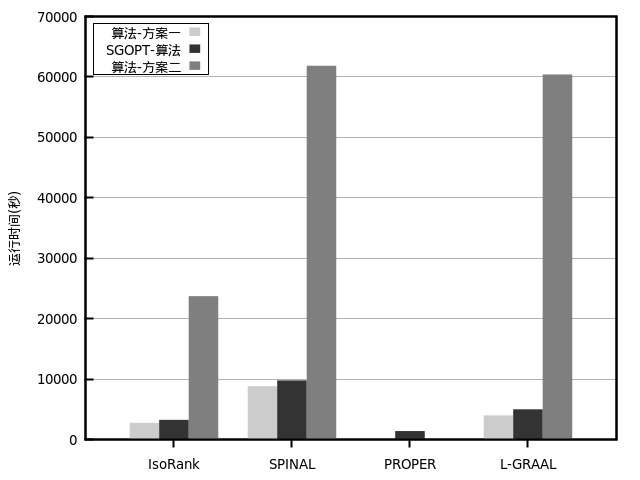
\includegraphics[width=\linewidth]{pic/dm-hs-Time.png}
            \label{dm-hs-Time}
        \end{minipage}
    }
    \caption{在\textit{dm-hs}实验组下,四种静态算法在三种方案下的实验结果。}
    \label{dm-hs}
\end{figure}

\begin{figure}[htbp]
    \subfigure[CE指标]{
        \begin{minipage}[b]{0.5\linewidth}
            \centering
            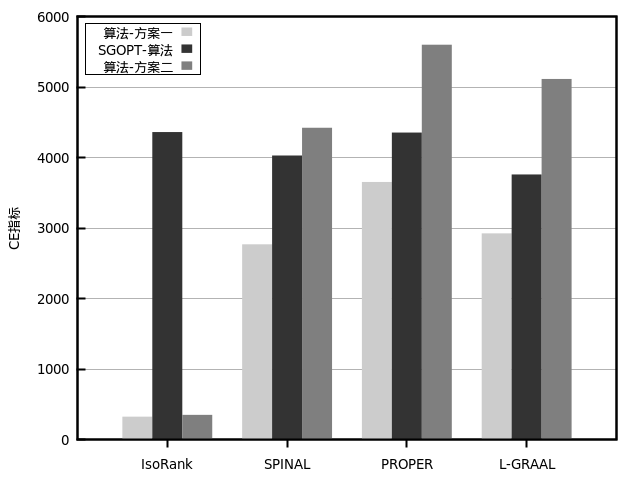
\includegraphics[width=\linewidth]{pic/dm-sc-CE.png}
            \label{dm-sc-CE}
        \end{minipage}
    }
   \subfigure[运行时间]{
        \begin{minipage}[b]{0.5\linewidth}
            \centering
            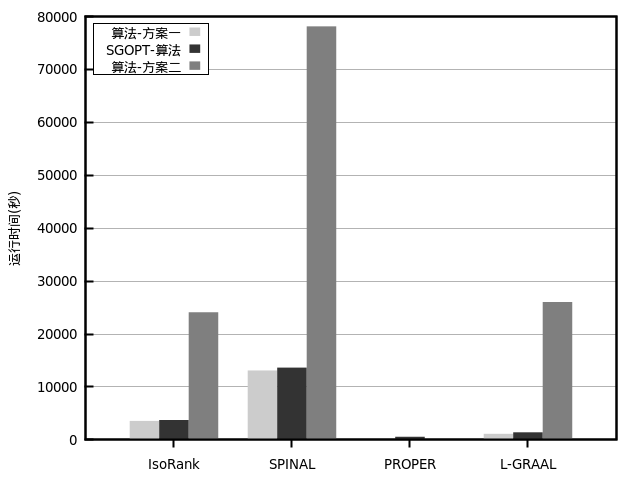
\includegraphics[width=\linewidth]{pic/dm-sc-Time.png}
            \label{dm-sc-Time}
        \end{minipage}
    }
    \caption{在\textit{dm-sc}实验组下,四种静态算法在三种方案下的实验结果。}
    \label{dm-sc}
\end{figure}

\begin{figure}[htbp]
    \subfigure[CE指标]{
        \begin{minipage}[b]{0.5\linewidth}
            \centering
            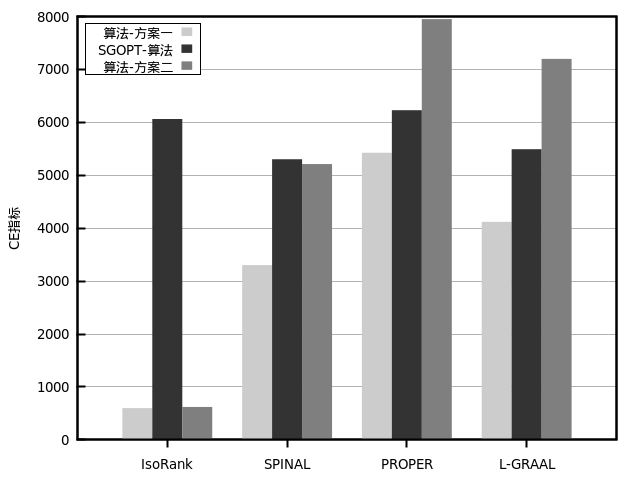
\includegraphics[width=\linewidth]{pic/hs-sc-CE.png}
            \label{hs-sc-CE}
        \end{minipage}
    }
   \subfigure[运行时间]{
        \begin{minipage}[b]{0.5\linewidth}
            \centering
            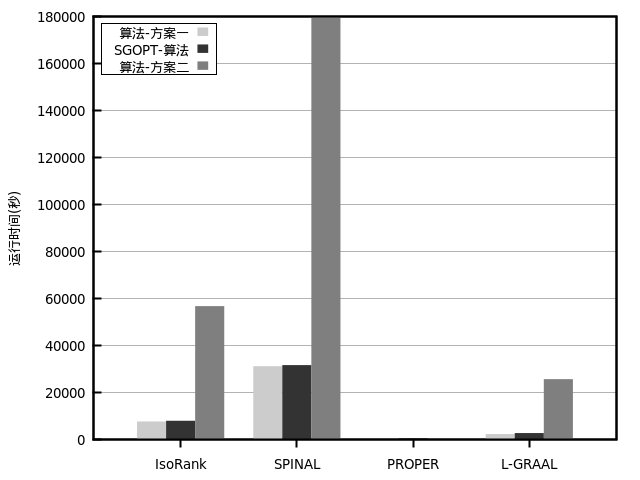
\includegraphics[width=\linewidth]{pic/hs-sc-Time.png}
            \label{hs-sc-Time}
        \end{minipage}
    }
    \caption{在\textit{hs-sc}实验组下,四种静态算法在三种方案下的实验结果。}
    \label{hs-sc}
\end{figure}

\subsection{CE指标的提高程度}
SGOPT算法对于四种比对算法在不同实验组下,对CE指标的优化的结果见图\ref{improveCE}。可以看到SGOPT对IsoRank的优化超出了预期,对于其他三种算法,SGOPT能够优化20\%到60\%。可见SGOPT是一种行而有效的优化框架。
\begin{figure}[!htbp]
    \centering
    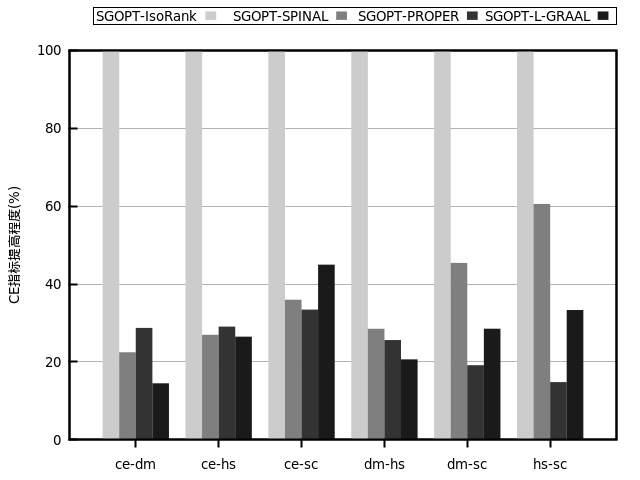
\includegraphics[width=0.8\linewidth]{pic/improveCE.png}
    \caption{在不同实验组下,SGOPT对于四种比对算法的CE指标的提高程度}
    \label{improveCE}
\end{figure}

%@@@@@@@@@@@@@@@@@@@@@@@@@@@@@@@@@@@@@2
\section{DEC,DICS,$DS^3$,DTWEC指标的对比}
目前为止所有的实验采用的衡量指标都是CE指标,那么在另外的指标下,SGOPT算法的效果又如何呢?图\ref{improveOther}是SGOPT算法对于其他指标的优化效果。

从不同的比对算法来看,对于IsoRank和SPINAL,可以看到SGOPT在所有实验组下都能对四项指标进行一定程度的优化。对于IsoRank,优化程度是超出预期的好,对于SPINAL,优化程度从20\%到60\%不等。在实验组\textit{hs-sc}中,对SPINAL的优化效果最好。而对于PROPER和L-GRAAL算法,SGOPT的优化效果则不如前两者。并且,SGOPT对于DICS和DS$^3$指标在实验组\textit{ce-dm,ce-hs,ce-hs,dm-hs}下没有任何优化效果。

从不同的衡量指标来看,DEC指标的优化效果最好,接下来的则是DTWEC指标,剩下的两个指标的优化程度则较差。

从不同实验组来看,可以发现在实验组\textit{dm-hs,dm-sc,hs-sc}下,SGOPT的优化效果教其他实验组好,猜想这是因为SGOPT的目标是最大化保留边的数目,而这一指标在两个网络都拥有很多边的情况下,会有更好的优化空间,所以结果也会较好。

\begin{figure}[!t]
    \subfigure[DEC指标提高程度]{
        \begin{minipage}[b]{0.5\linewidth}
            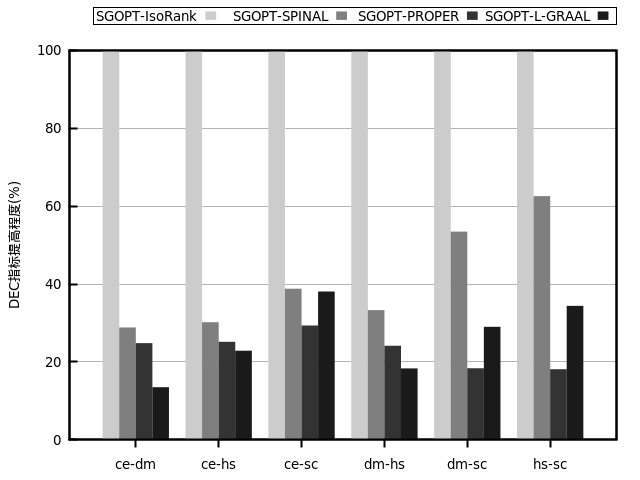
\includegraphics[width=\linewidth]{pic/improveDEC.png}
            \label{improveDEC}
        \end{minipage}
    }
   \subfigure[DICS指标提高程度]{
        \begin{minipage}[b]{0.5\linewidth}
            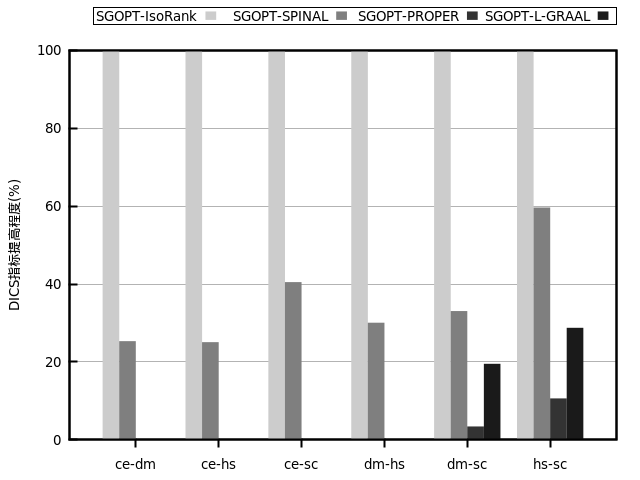
\includegraphics[width=\linewidth]{pic/improveDICS.png}
            \label{improveDICS}
        \end{minipage}
    }
     \subfigure[DS$^3$指标提高程度]{
        \begin{minipage}[b]{0.5\linewidth}
            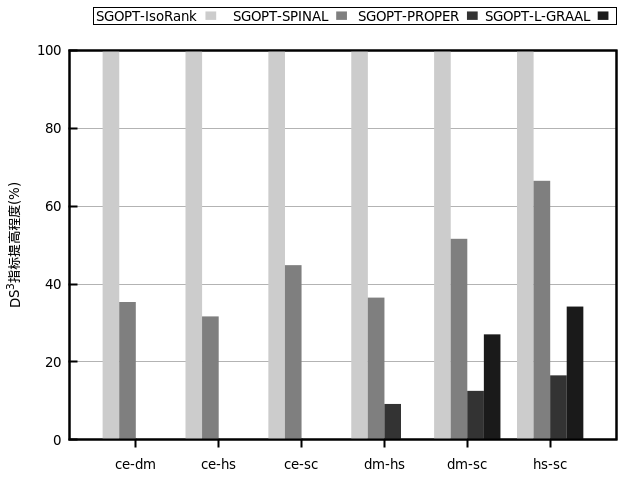
\includegraphics[width=\linewidth]{pic/improveDS3.png}
            \label{improveDS3}
        \end{minipage}
    }
     \subfigure[DTWEC指标提高程度]{
        \begin{minipage}[b]{0.5\linewidth}
            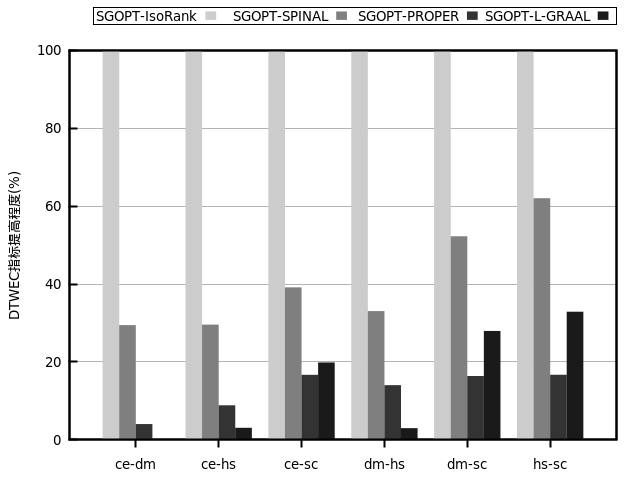
\includegraphics[width=\linewidth]{pic/improveDTWEC.png}
            \label{improveDTWEC}
        \end{minipage}
    }
    \caption{SGOPT算法对于其他四项指标的优化效果}
    \label{improveOther}
\end{figure}



\chapter{总结与展望}

本文着眼于PPI网络匹配的问题,提出了动态PPI网络这一概念,在该概念下,提出了动态PPI网络匹配这一新问题的定义,并且提出了基于线段树数据结构优化的SGOPT算法,该算法能与目前所有的静态PPI网络全局匹配算法结合,在动态PPI网络这一环境下,优化并提高匹配的效果。SGOPT算法以CE\ref{myworkmaxfidefine}值作为优化目标,利用线段树能够快速更新动态匹配的能力,以一种局部随机调整的策略,大大优化了既有算法的匹配效果,大量的实验也证实了该算法的可行性和可用性。

由于本文是对PPI动态网络匹配这一新问题的初次尝试,考虑的问题是一静一动的网络匹配模式,但是两个动态PPI网络匹配的问题,相对于本文,应该更具有现实意义,在两个动态PPI网络上进行网络匹配,必定也是一个值得尝试与研究的新课题。
\rhead{总结与展望}

\song
\rhead{参考文献}
\addcontentsline{toc}{chapter}{参考文献}

\bibliographystyle{unsrt} %引用方式
\bibliography{cite}
%\chapter*{学术论文}
\rhead{学术论文}
\addcontentsline{toc}{chapter}{学术论文}

\textbf{发表论文}
\begin{enumerate}
\item \textbf{XXXX},XXXX
\end{enumerate}
\chapter*{致谢}
\rhead{致谢}

时间转瞬即逝,一转眼,作为一个复旦计算机研究生的三年生涯,即将引来最后的时刻。三年来的研究生学习与生活,无疑是对刚本科毕业时的我的一番锤炼与鞭策,此刻的我深深感受到了三年来自己逐步发生的蜕变。而这一切无疑离不开导师,同学与家人的影响。

三年的研究生生涯,对自己影响最深的,必定是自己的研究生导师了。我要感谢我的导师周水庚教授在三年里对自己的谆谆教导,无论是学术方面还是生活方面。三年里的每一次的学习机会,无疑都是周老师给予我的,从中我学到了很多,也体会到了很多。都说工作了的人会怀念自己的学生生涯,我想就算以后步入职场,也必定常会感念周老师的教导。

都说研究生的生活有时会显得枯燥乏味,然而有同学们和朋友们在自己的身旁,感觉有时显得枯燥的生活也有了如绚丽色彩般的点缀。除却良师,便是益友。无论是上一届的学长学姐们,还是同一届的同学朋友,亦或是下一届的学弟学妹们,他们的帮助,都是对自己研究生生活最好的鼓励,感谢他们所做的一切。

当然,研究生生活也少不了家人们一如既往的支持。虽然研究生生活少不了挫折困难,也遭遇过失望难受,但是一想到有家人作为自己的后盾,有温暖的亲情支撑着自己,就觉得什么都是值得的了。感谢自己的父母,也为拥有这样的父母而感到幸运。

愿我们都能在以后的生活中,将现在的一切都铭刻于心,不忘青春,不忘初心。
\addcontentsline{toc}{chapter}{致谢}

\end{document}